\chapter{基于时延的集中式段路由航点生成算法}

\section{引言}

本章将以集中式软件定义网络控制器的视角对基于时延的段路由航点生成算法进行问题建模分析,对链路权重公式和辅助图生成的核心算法进行详细阐释,并分析算法的时间复杂度。

\section{问题模型}

段路由网络中具有非段路由节点和段路由节点,控制器通过带外控制链路和段路由节点通信,控制器需要分配、通告段路由标签,并按照到达数据包的时延需求计算段标签列表,如图3-1所示。将网络中的交换机抽象成节点,链路抽象成双向有向边,构成有向图$G(V, E)$。假设任何一个节点$v$都有可能有流量到来,$f(s, d)$ 表示源节点为$s$,目的节点为$d$的待服务流量,在真实IP网络中,一般用源地址、目的地址、源端口、目的端口、协议组成的五元组来标识一个流量,但是在问题建模中,不需要考虑传输层的端口号和具体协议号,因此只需要用源地址、目的地址 $f(s, d)$ 来标识一条流量。

\begin{figure}[htbp]
\setlength{\abovecaptionskip}{15pt plus 3pt minus 2pt}
\centerline{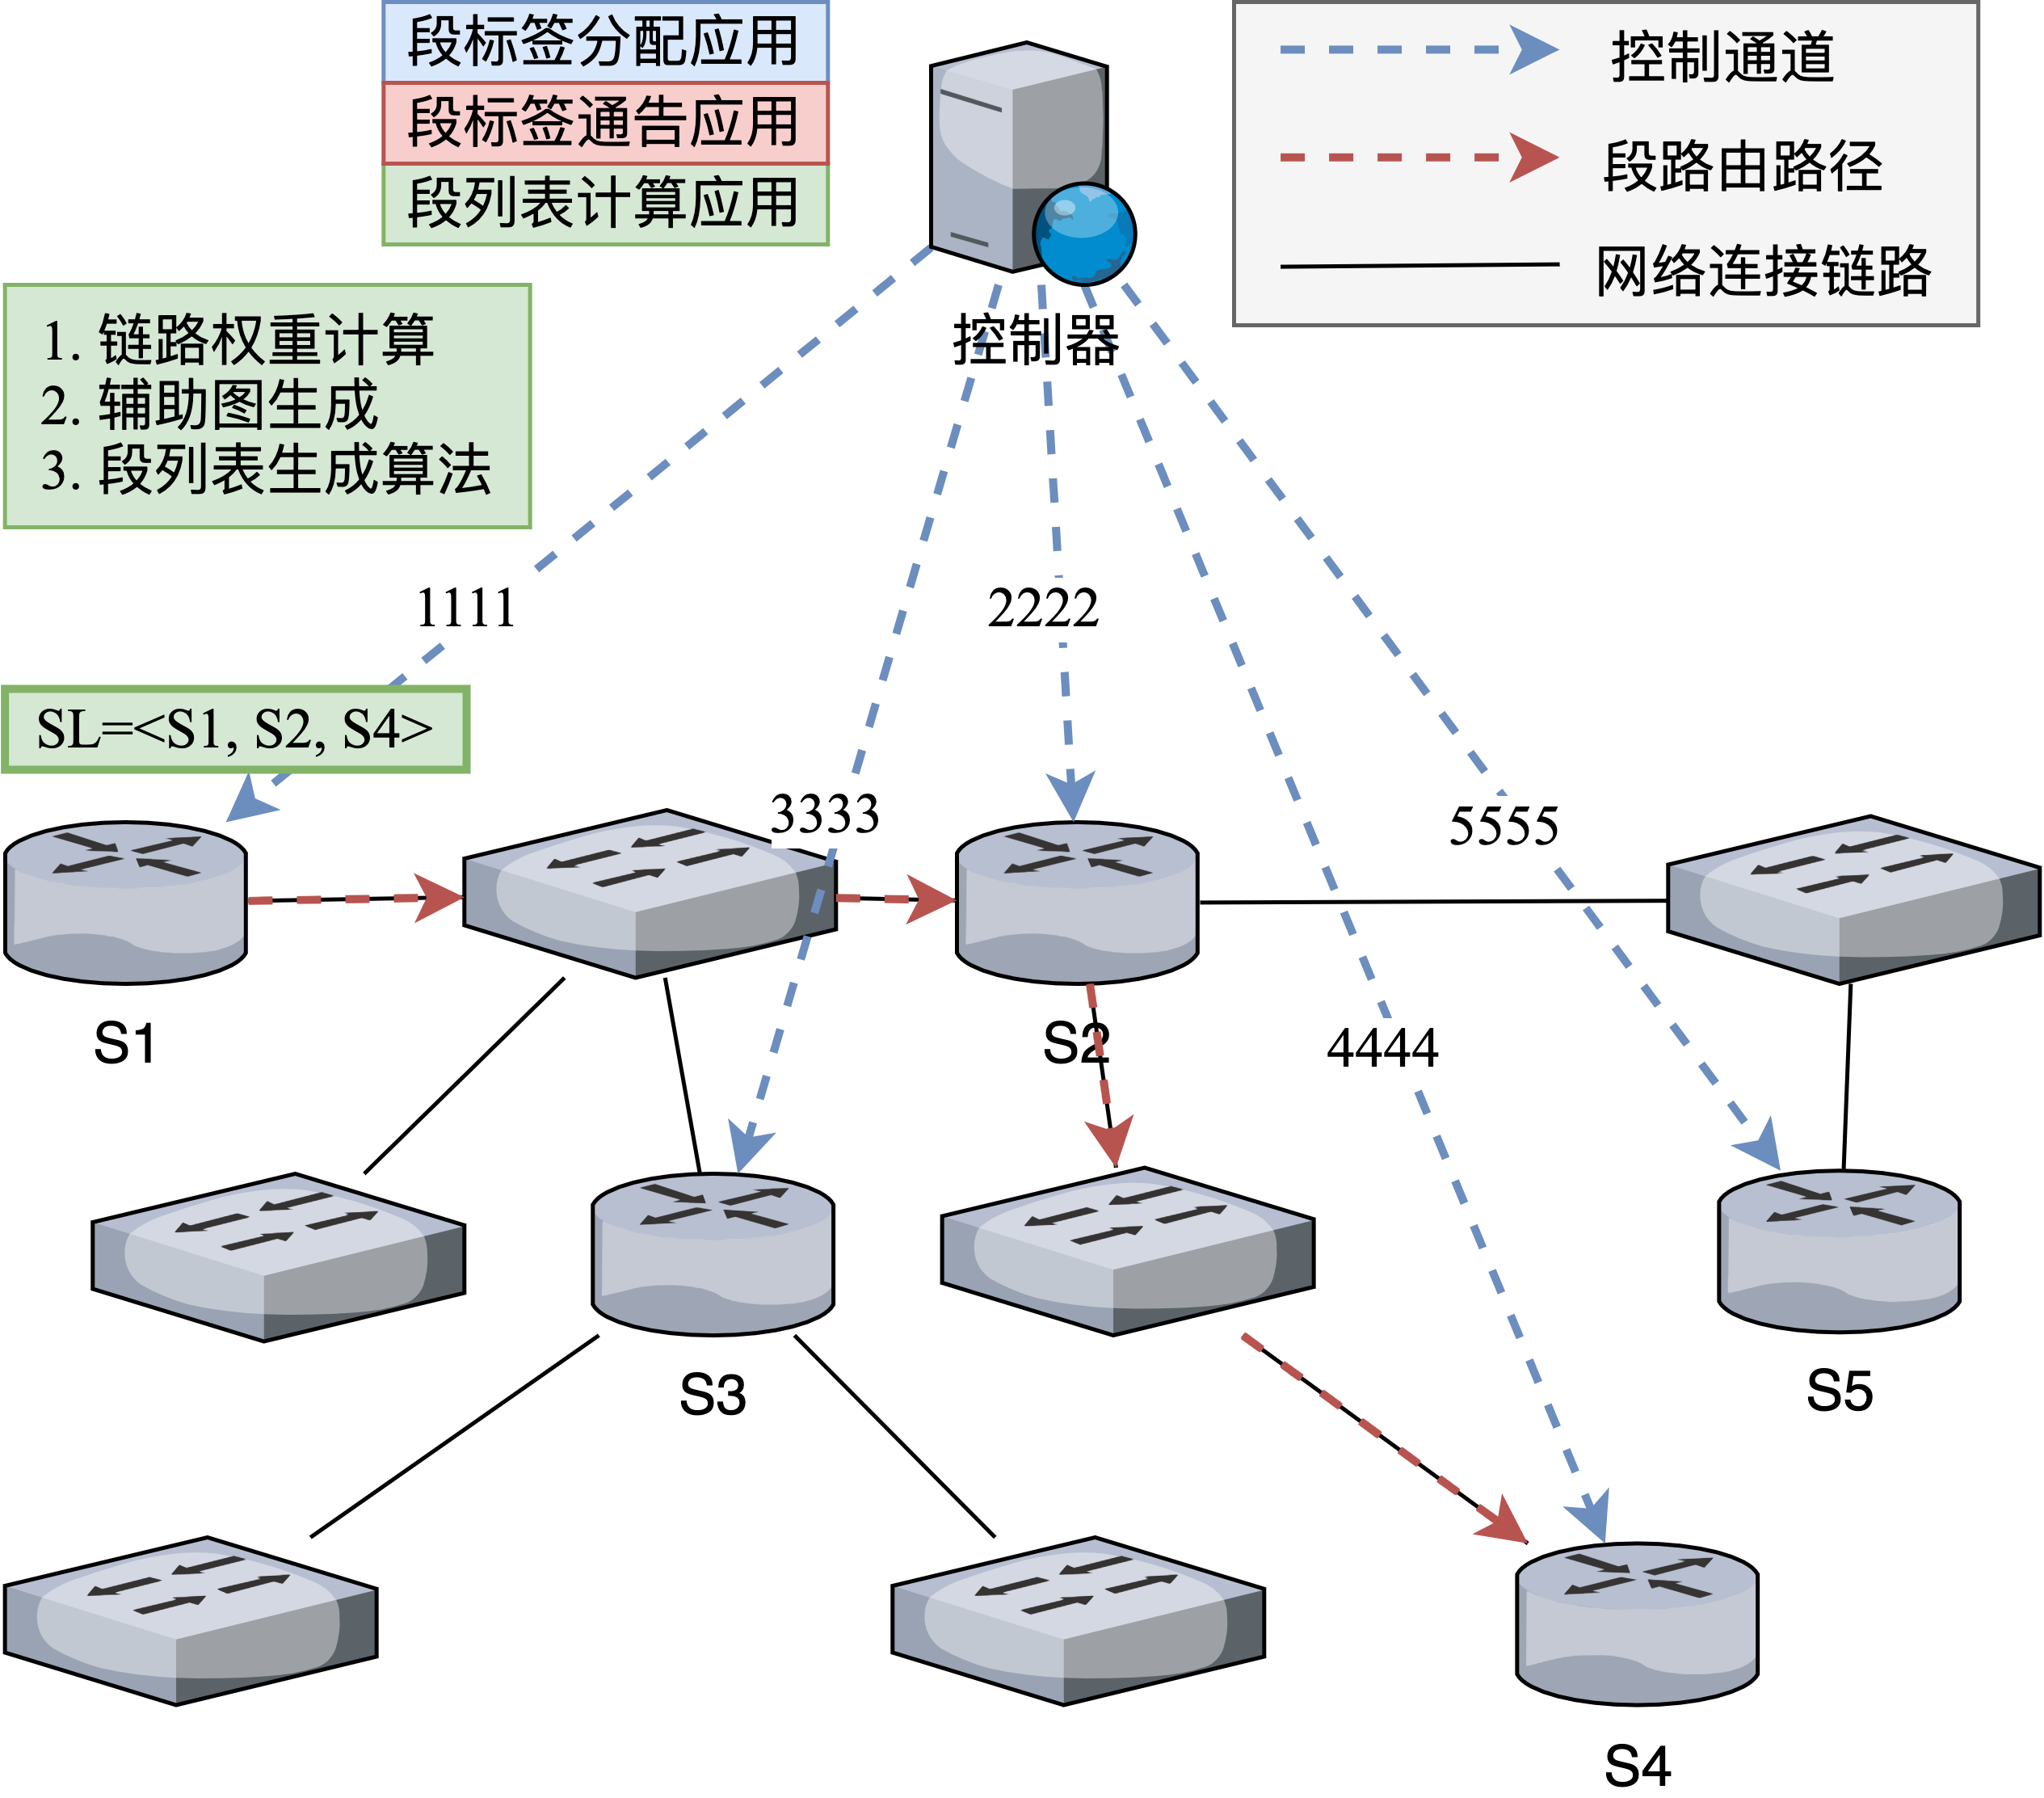
\includegraphics[width=0.8\textwidth]{./figures/ch3-problem-model.png}}
\caption{集中式段路由控制面问题模型}
\label{fig-ch3-problem-model}
\end{figure}

因此将问题建模为:已知有向图$G(V, E)$,流量$f(s, d)$,计算出一组段标签,使得流量通过这组段标签的时延较短。

\section{基于时延的段路由航点生成算法}

\subsection{算法概述}

段路由航点生成算法本质上是一个最优路径选择问题。在弱约束的情况下,最优路径选择是一个完全非确定多项式(Complete Nondeterministic Polynomial, NP-complete)问题。在研究基于软件定义网络的广域网中的段路由流量工程的文献中 \cite{SRBANDWIDTH8} ,并证明一般的段路由标签列表选择问题是一个非确定多项式难题(Hard Nondeterministic Polynomial, NP-hard),非确定多项式难题代表如果解决一个问题的算法可以转化为解决任何非确定多项式问题的算法,那么这个问题就是非确定多项式难题。即非确定多项式难题意味着“至少和任何非确定多项式一样难”。如果段路由只允许每条路径有固定数量的$M$个中间点,那么具有最短路径的流量工程是弱多项式可计算的。覆盖面最广的方法是将所有节点视为候选中间点,将网络拓扑中的全部节点标记为V,候选节点标记为$C$,则有$C = V$。然而这会导致解决一个流量工程资源分配问题的程序的成本会非常高昂。另一种方法是只考虑少量的中间节点,例如$C=k \cdot |V|$,这里$k$是一个比例系数,虽然只是使用了一部分全部网络拓扑的节点进行计算,这仍然会为流量工程的需求输出出性能良好的方案。这里提到的中心度概念只是关注网络拓扑图结构的结构度量,即各个节点之间的连接关系。在一些研究 \cite{SRBANDWIDTH9} 中表明当中间点的数量固定而不是输入的一部分时,流量工程路径问题可以在弱多项式时间内解决。但是如果有固定的参数来约束,该问题可以在多项式时间内解决。因此段路由标签列表的长度被用来限制研究中的段列表生成算法。一般来说,深度为2的段列表可以有更好的流量分流效果。在一些文献中作者分析了现实世界的流量 \cite{2SR} ,并扩展了2-段路由公式,以最小化非最短路径隧道的数量。他们还评估了3-段路由和4-段路由的流量工程能力,表明它们非常耗时。因此在本研究中,段路由标签列表的长度被限制为2或3,段列表长度的影响在实验中得到了验证。最后贝尔曼-福特算法将被用于计算段路由标签列表基于上述问题的建模和限制条件。

总结上述内容,本章将讨论的主体有两个部分,第一个是如何设计出考虑时延状态的链路权重计算公式,第二个是如何优化原本为非确定多项式难题的段路由航点生成算法。问题一将在3.3.2进行讨论,问题二的优化方法则是分为两个部分,第一个是如何选择少量的节点基于具有多项式复杂度的替代中心度度量的实用中间点选择,解决这个问题的方法是辅助图生成,将在3.3.3进行讨论,第二个问题则是如何限制最优路径选择问题中的迭代次数问题,使其从非确定多项式难题转变为多项式时间解决问题,这个问题的解决方案是限制段标签列表的深度,将在3.3.4进行讨论。

\begin{figure}[htbp]
\setlength{\abovecaptionskip}{15pt plus 3pt minus 2pt}
\centerline{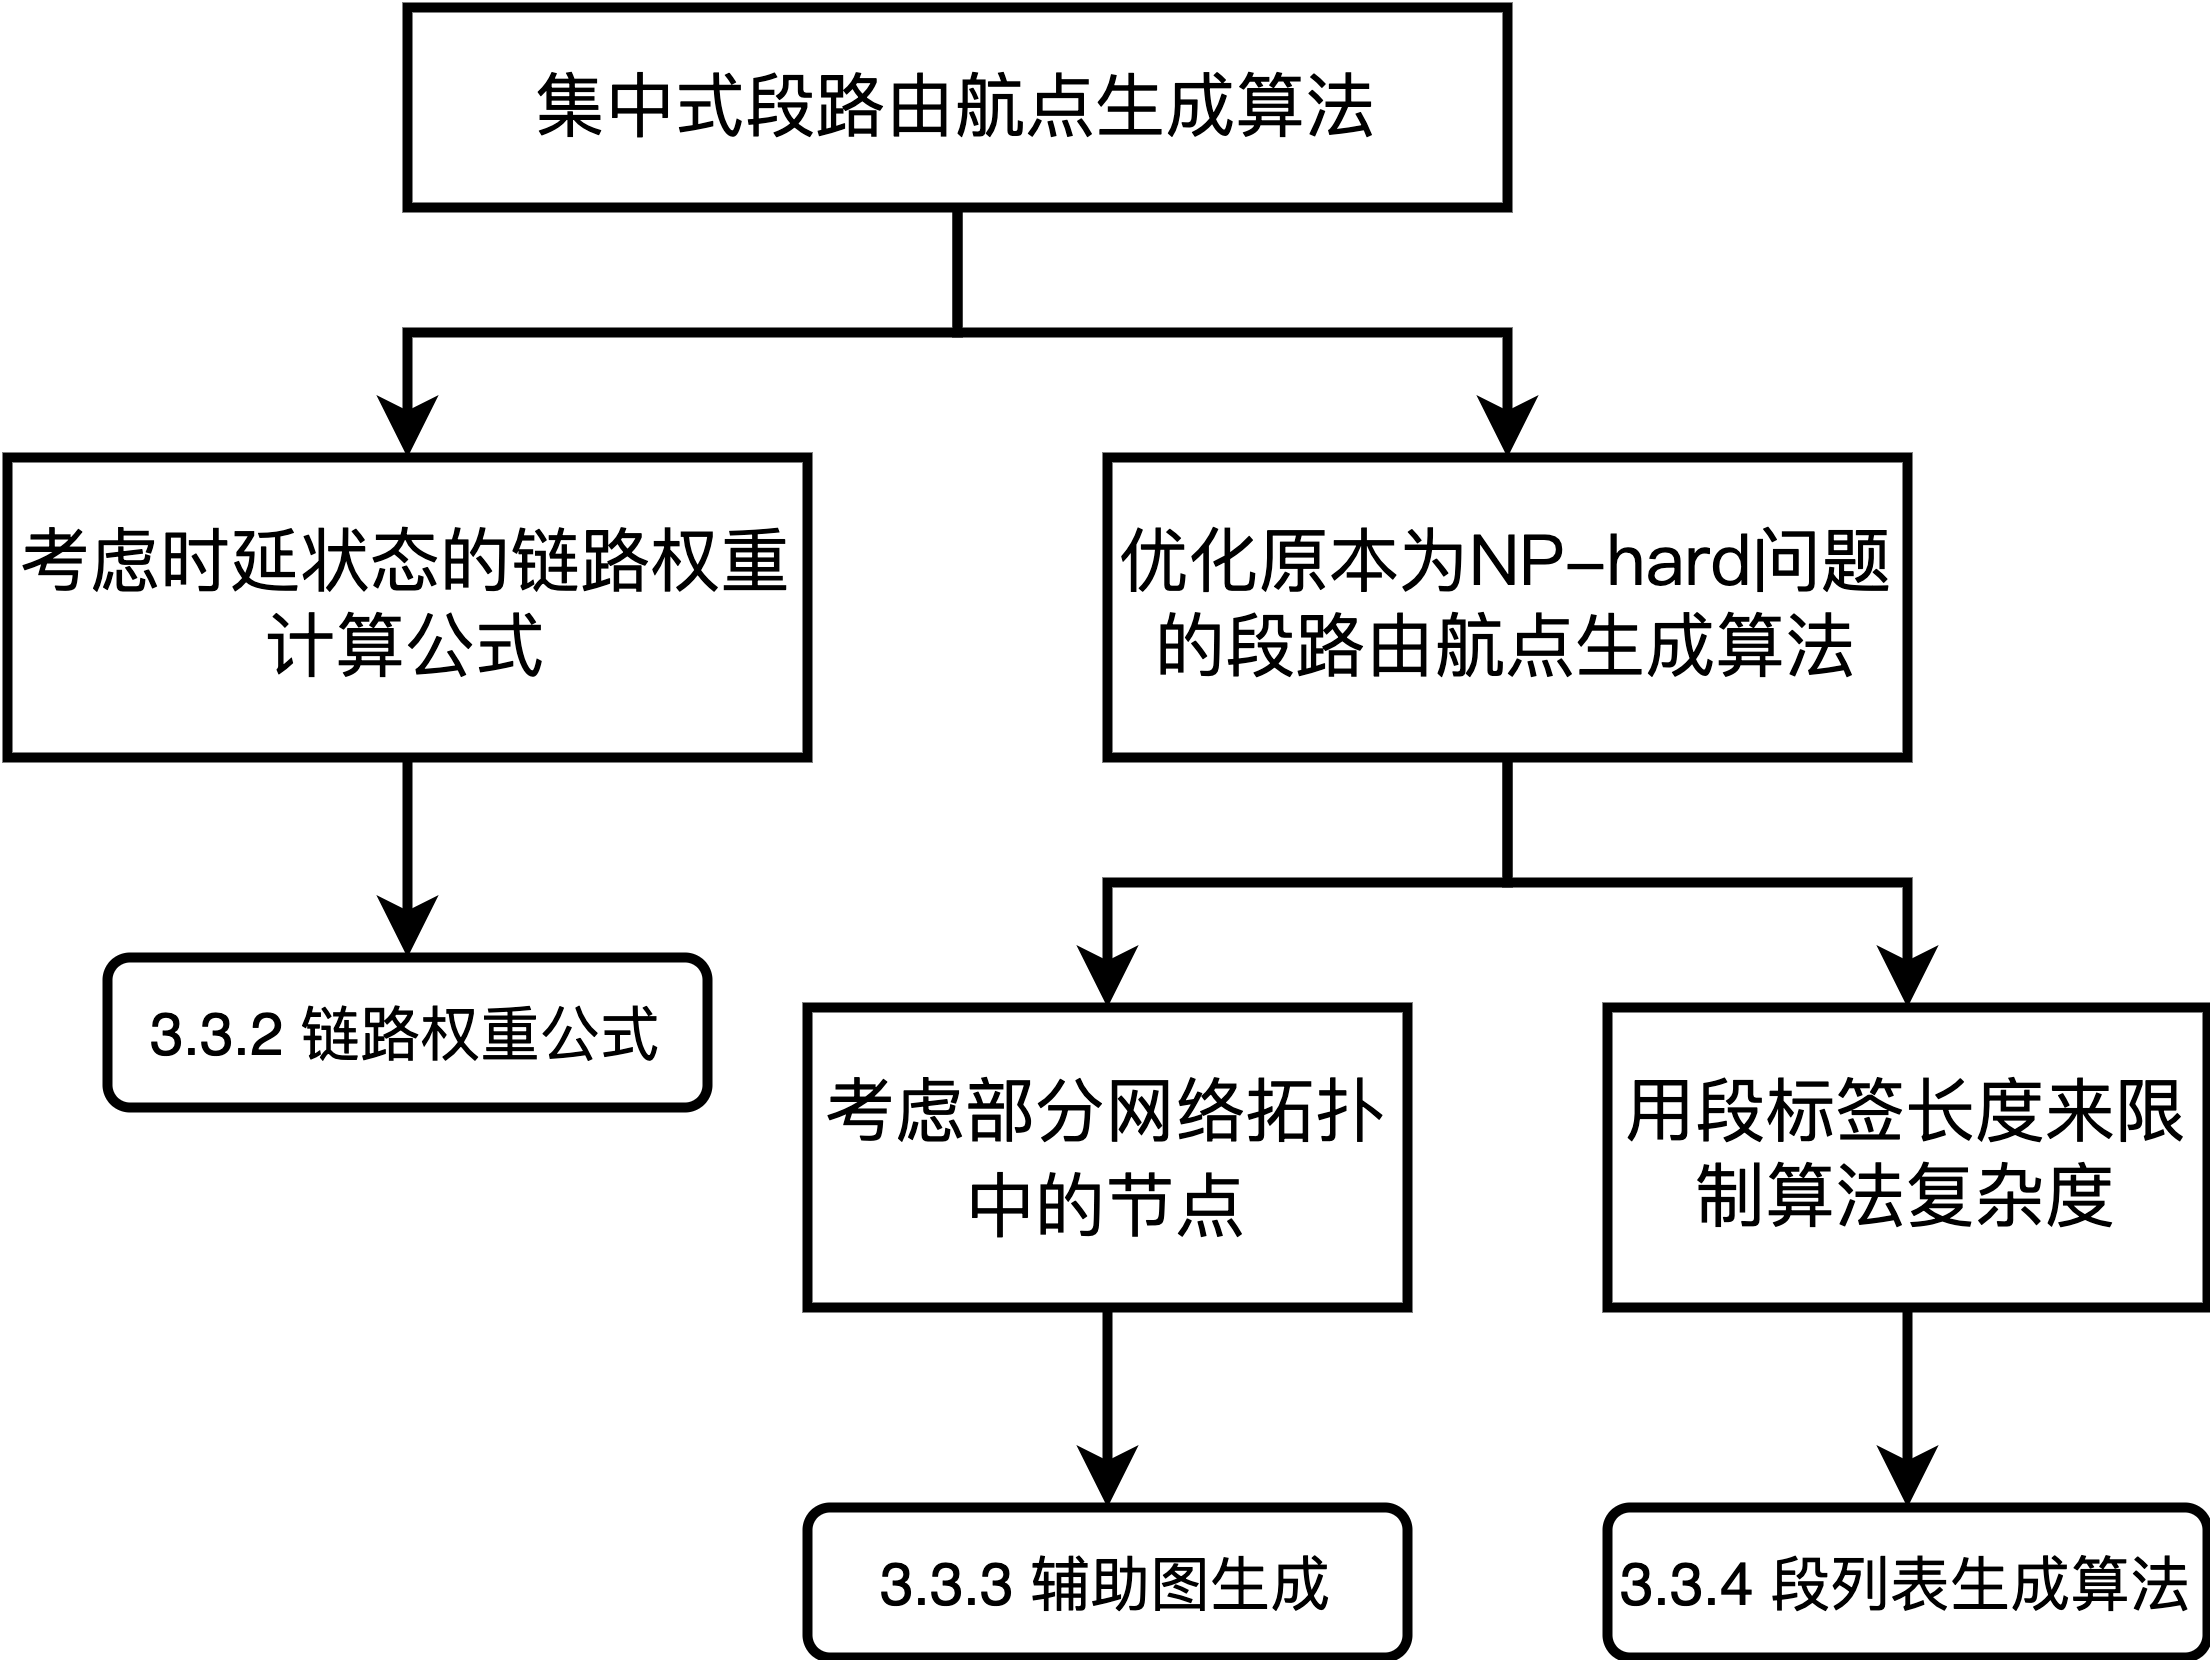
\includegraphics[width=0.8\textwidth]{./figures/ch3-ark.png}}
\caption{集中式段路由航点列表生成算法思路索引结构图}
\label{fig-ch3-ark}
\end{figure}

对于基于时延段路由的航点生成算法来说,主要步骤有三步:第一步是静态场景下计算链路权重,第二步是在原有拓扑上生成拓扑数目为了将时延更好地结合到节点选择的算法中,本文没有直接将通常用带宽进行估算和权重衡量的方案直接替换成采集到的时延参数,而是将时延信息和带宽进行综合分析并构建出权重公式。基于构建出的权重公式在较为静态的网络环境下计算各个链路的权重。并且在基于静态情况下对网络节点的权重进行计算,选择相对较为核心的节点构造辅助图,辅助图将是节点选择算法中选择节点对象的集合,这是因为选择中心度更高的节点在调流上会达到更好的效果。试想如果一个节点被各种情况下经过的概率更高,那么选择其他节点也都会有更大的概率达到这个节点,辅助图节点集合的确定就是为了缩小节点选择范围使得后期遍历的算法复杂度降低。最后本章通过贝尔曼-福特算法得出段路由需要的航点列表,选择贝尔曼-福特算法而非迪杰斯特拉等最短路径算法的原因主要是考虑到负权重路径的存在。

本节剩下的章节将对以上提到的三个算法点进行详细的解释。

\subsection{链路权重公式}

通常来说,网络流量图以及流量工程矩阵都是以带宽为度量数据的,因此在有向图$G(V, E)$中如何考虑时延制定有向边的的权重是第一个需要明确的问题。在本节中,本文考虑到拓扑因素、延迟效应和带宽限制,从这三个角度构建了一个通用衡量的链路权重的表达式。

1. 链路中心度

本文用链路中心度量化拓扑因素。已知$(s,d)$表示网络中可能产生通信需求的源节点和目的节点,则令$S_{sd}^k$表示这一对源节点和目的节点$(s,d)$之间前k条最短路线的集合。令$e$表示网络中的每条有向链路,令$f_{sd}^k(e)$表示链路$e$在源节点$s$到目的节点$d$的前$k$条最短路线路径中出现的频率。

基于上述定义,$f_{sd}^k(e)/k$可以被视为$(s,d)$之间前$k$条最短路径中链路$e$的出现率。因此,本文计算流量矩阵中可能产生通信的每一对节点之间的前k条最短路径,并将$e$出现的频率相加。这个频率的总和用于确定网络中链接$e$的中心度,它的含义是在链路$e$在各种网络层路由算法中被选中的可能性,因此链路$e$的链路中心度$c(e)$使用各个节点对的$f_{sd}^k(e)/k$的累积加和来计算。相对于流量变化的频率,网络拓扑从结构上来看基本是处于静态的。因此,本算法需要在静态阶段针对网络中所有可能的通信路径,用如迪杰斯特拉等最短路径算法计算出$(s,d)$的前$k$条最短路径,这个时间复杂度是$|V|\cdot O({|E|}^2)$。但是链路中心度并不是需要一直计算的,只有在网络拓扑出现变化的时候才需要更新,可以说这个参数是事件驱动的,并不会长时间占用控制器的计算资源。因此可以用公式3-1计算链路中心度。

\begin{equation} \label{link centrality}
    c\left(e\right)=\sum_{\forall(s,\ d)\in T M}{f_{sd}^k\left(e\right)}/k
\end{equation}

设计链接中心度$c(e)$的意图是表征等价多路径路由选择特定链接$e$的可能性,等价多路径路由常用于IP网络中作负载平衡,只要路径跳数相等即视为等价,就可以流量在这些路径上负载均衡。因此$c(e)$越大,任何两点产生通信时,数据流量通过$e$的概率也就越大。

2. 链路到达率

从本质上讲,交换机端口的排队延迟是由于数据包的到达但没有得到及时处理而造成的。根据排队理论中对任何到达和服务分布都成立的利特尔法则(Little's law):$W_q=L_q/\lambda$,可以得到以下推断。

在利特尔法则中$W_q$是排队问题的平均等待时间,$L_q$是平均队列长度,$\lambda$是到达率。到达率衡量的是顾客进入队列的速度。经过转换利特尔法则,就可以得到$\lambda$的计算公式。$\lambda=W_q/L_q$。此外,当到达率小于服务率时,排队系统可以得到平衡。

交换机模型中的平均队列长度$L_q$可以用单位时间内通过定向链路$e$的数据包数量来衡量,定向链路实际上就是交换机端口发送的 \gls*{PPS} ,用$p(e)$表示。平均等待时间$W_q$可以用交换机中消息元数据的时间戳来计算。例如,在 \gls*{PISA} 中,$standard\_metadata.ingress\_global\_timestamp$在入口管道开始解析消息并将其添加到消息的原始头中之前使用。为了记录消息到达时间戳的元数据,$standard\_metadata.egress\_global\_timestamp$是在出口管道开始解析消息之前添加在消息的原始头之前的元数据,用来记录消息通过流量管理器到达出口时的时间戳。由于排队的数据包几乎都发生在流量管理器中,这两个元数据的差异可以用来衡量数据包的排队延迟。在交换机中进行统计平均后,可以收集并计算出$W_q$,记录为$d(e)$。因此,交换机中的链路到达率$\lambda(e)$可以用公式3-2计算:

\begin{equation} \label{link arrival rate}
    \lambda(e)\ =\ p(e)/d(e)
\end{equation}

链路到达率$\lambda(e)$背后的含义是表示未来短时间内是否有大量数据包会到达某条链路$e$上。由于网络中的预测信息是根据历史数据推断出来的,$\lambda(e)$越大,未来需要在链路$e$上服务的到达数据包就越多,排队的可能性也就越大。

3. 链路拥塞度

带宽是计算链路权重时必须考虑的一个问题。带宽和延迟不成比例的一个重要原因是,交换机中的队列只是数据包的头,而不是整个数据包。整个数据包的大小与数据包头的大小无关,这意味着一条链路可能被阻断。小数据包填满了缓冲区,但实际带宽并不反映高负荷。同样,一条链路可能被大数据包填满,缓冲区没有排队或延迟,但链路带宽可能真的有瓶颈。因此,有必要考虑链路$e$的当前负载是否会影响未来的路由性能。

让$f(e)$表示链路$e$的已用带宽,让$b(e)$表示链路$e$的总带宽,让$r(e)$表示链路$e$的剩余带宽,即,$r(e)=b(e)-f(e)$。

基于上述定义,构建的链路负载率$s(e)$表示链路$e$使用带宽的比例,计算公式如公式3-3所示:

\begin{equation} \label{link congestion}
    s(e)\ =\ f(e)/r(e)
\end{equation}

链接拥堵指数$s(e)$的定义是一个增加的凸函数。也就是说,$s(e)$越大的链路意味着流量很可能立即爆满,需要避开。

4. 链路权重

为了结合上述三个参数来计算与延迟有关的定向链路的权重,首先应该考虑这些参数的特点。
$c(e)$与拓扑状态和$k$的值有关。当$k=1$时,数值范围可以达到$(0,\ count(V_{Host})/2),count(V_{Host})$是网络中可能发起消息的主机节点数量;当$k>1$时,数值范围的上限应该小于$count(V_{Host})/2$。这意味着$c(e)$是一个幅度不太大的参数,它比$\lambda(e)$和$s(e)$的值更固定。

$\lambda(e)$是排队到达率,它与到达交换机的数据包大小有关。根据对数据中心网络情况的观察,$\lambda(e)$的大小在$({10}^5,{10}^8)$之间。为了反映排队到达的计算效果,该值需要接近$s(e)$,所以取$\lambda(e)$的对数,使其接近$s(e)$和$c(e)$。

$s(e)$是一个递增的凸函数,其数值范围为$\left(0,\infty\right)$。当$f(e)$极小时,$s(e)$接近0,$\lambda(e)$会比以前小一点。所以要平衡$s(e)$和$\lambda(e)$的变化。$\lambda(e)$取$10$的对数,得到$\left(5,\ 8\right)$的值,为了增加其影响力,用它作为$s(e)$的指数来参与计算。最后,考虑影响范围,将$c(e)$的权重考虑在内,最后得到有延时的有向链接$w(e)$的权重。

值得一提的是,在链路权重的设计过程中,本文考虑了两种情况。

第一种是当链路完全不拥塞的时候,着重考虑链路中心度,而当链路产生拥塞的时候,考虑链路拥塞度和链路到达率,这种设计方案,需要一个额外的参数来调和这几个参数相加时的比例,例如公式3-4:

\begin{equation} \label{first link weight equation}
    w(e)=\theta \cdot s(e)ln(λ(e)) +(1- \theta )/c(e) \ \  0 \le \theta \le 1
\end{equation}

第二种利用链路拥塞度的凸函数激增特性,当链路不拥塞的时候,着重考虑链路中心度,而当链路产生拥塞的时候考虑链路到达率,在这其中用链路拥塞度来作为调和比重的参数,由于该参数需要用归一化的方式调和,因此将$s(e)/100$和$1-s(e)/100$作为调和$c(e)$和$\lambda(e)$的系数,如公式3-5所示:

\begin{equation} \label{second link weight equation}
    w(e) = c(e) \cdot (e)/100 + \lambda(e) \cdot (1-s(e)/100)
\end{equation}

下文将对这两种构造方法进行比较得出最终使用的链路权重公式。

当考虑第一种算法时,目的是当链路完全不拥塞的时候,着重考虑链路中心度,而当链路产生拥塞的时候,考虑链路拥塞度和链路到达率。所以将几个不重要的参数设置为常量,其中$e$是一个有向链接,$\theta$是调整链接属性和链接状态的系数。$\theta$是一个保留参数,在后面对此公式3-4进行分析的实验计算中都取为$0.5$。如何为$\theta$取一个更合适的值,需要根据具体的网络进行调整,因为它对平衡链接属性和链接状态很有用。公式3-4建议使用临界度较高的链路和具有更多可用带宽和较低链路到达率的链路。因此假定到达率$\lambda\left(e\right)$为$0.5$,$\theta$为$0.5$。对于一个给定的链路$c\left(e\right)$是一个常数,所以随着链路流量的逐渐增加,链路权重的增加趋势如图3-3所示。

\begin{figure}[htbp]
\setlength{\abovecaptionskip}{15pt plus 3pt minus 2pt}
\centerline{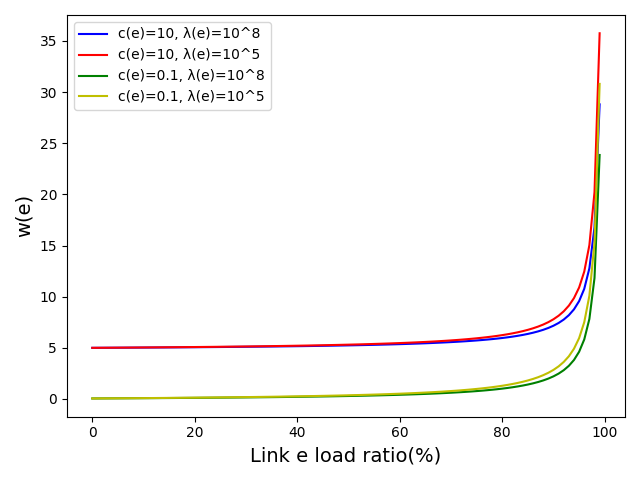
\includegraphics[width=0.8\textwidth]{./figures/ch3-link-weight-function-1.png}}
\caption{第一种链路权重算法下链路权重随链路负载增长变化示意图}
\label{fig-ch3-link-weight-function-1}
\end{figure}

当网络负载较轻时,链路可用带宽和链路到达率都很低,权重函数倾向于参考链路临界值$c\left(e\right)$;当网络负载较重时,链路可用带宽和链路到达率较高,链路权重函数会急剧增加,因此权重函数会倾向于参考链路拥塞指数$s\left(e\right)$和链路到达率$\lambda\left(e\right)$。当网络资源利用饱和时,通过链路拥塞指数$s\left(e\right)$和链路到达率$\lambda\left(e\right)$来确定链路权重是合理的,而不是在拓扑属性下确定链路临界度。

当考虑第二种算法时,目的是当链路几乎不拥塞的时候,着重考虑链路中心度,而当链路产生拥塞的时候,重点考虑链路到达率。这样做是考虑到当链路几乎不拥塞的时候,具有更高链路中心度的链路是可以提供更高联通度的链路,本身就更容易在IP层的哈希中被选中。而当链路产生拥塞的时候,该算法希望能选出那些未来数据包到达率更低的链路,避免竞争。链路权重的增加趋势如图3-4所示。选择链路中心度分别为$0.5$、$0.01$的链路,假设数据包到达率不变分别为$0.5$和$0.01$,将它们两两组合,则可以画出在这4种情况下,使用公式3-5的链路链路权重随链路负载增加的情况。

\begin{figure}[htbp]
\setlength{\abovecaptionskip}{15pt plus 3pt minus 2pt}
\centerline{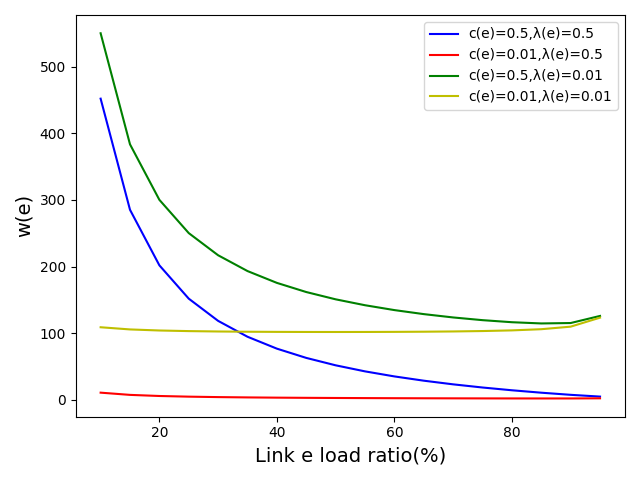
\includegraphics[width=0.8\textwidth]{./figures/ch3-link-weight-function-2.png}}
\caption{第二种链路权重算法下链路权重随链路负载增长变化示意图}
\label{fig-ch3-link-weight-function-2}
\end{figure}

只观察$c(e)=0.5,\ \lambda(e)=0.5$(蓝色折线),可以看出控制链路到达率不变,当网络负载较轻时,链路可用带宽较高,$c(e)=0.5$的链路具有较高的链路权重;当网络负载较重时,链路可用带宽低,链路拥塞度高,造成链路权重下降。

将$c(e)=0.5,\lambda(e)=0.5$(蓝色折线)和$c\left(e\right)=0.01,\lambda\left(e\right)=0.5$(红色折线)对比,控制链路到达率不变时,链路中心度较高的链路一直有较高的权重,而链路中心度较低的链路直到链路带宽基本占用满才和高链路中心度链路具有相同的链路权重。

将$c(e)=0.5,\lambda(e)=0.5$(蓝色折线)和$c\left(e\right)=0.01,\lambda\left(e\right)=0.01$(黄色折线)对比,当网络负载较轻时,权重函数倾向于选择链路中心度$c\left(e\right)$更高的链路,而当网络负载较重时,权重函数倾向于选择链路到达率$\lambda\left(e\right)$更低的链路。即当网络资源利用饱和时,链路拥塞指数$s\left(e\right)$已经很高了,此时通过链路到达率$\lambda\left(e\right)$来确定链路权重而不是用拓扑属性的链路中心度是合理的。

除此以外,方案一的权重函数,在链路中有中心度较高但到达率低的链路又可能不如链路中有中心度低但到达率高的链路权重,这也是不合理的地方,因此经过上问的分析,本算法使用方案二的链路权重函数作为考虑时延情况的链路权重函数。

在评估了链路权重$w\left(e\right)$后,在生成辅助图的边集过程中,权重$w\left(e\right)$小于$\beta$的链路将被删除。所以算法将设置一个阈值,表示为$\beta$,并在生成辅助图时设置$\beta=20$来限制一个链路权重的大小不能过小。

\subsection{辅助图生成}

由于段路由的节点集是整个节点集的一个子集,所以可以不把所有的链接和节点提到计算范畴,而是选择一些节点重建拓扑图,节点的选择主要考虑的是节点中心度,按原有拓扑节点总数的幂次比例的子集作为辅助图节点,进而通过链路属性的筛选来生成一个辅助图以降低拓扑复杂性和计算段标签列表生成的时间复杂度。

1. 节点中心度

本段将讨论基于具有多项式复杂度的替代中心度度量的实用中间点选择。值得注意的是,这些中心度是关于拓扑图本身结构的结构度量量,即主要通过各个节点之间的连接关系来评判中心度。因此这些节点中心度的计算方式一般没有考虑网络中存在流量的情况,也不会考虑网络流量守恒和容量约束等问题。这里将讨论三种节点中心度度量方式,分别是最短路径中心度、组最短路径中心度、度数中心度,评判三种常见中心度的侧重最终得出本文使用的节点中心度计算公式。

最短路径介数中心度根据随机选择的源-目的地址对,通过该节点v的最短路径的数量就是可以表征节点v的中心度的度量量。具体而言,假设在有向图$G=\left(V,E\right)$中,如公式3-6所示,节点$v \in V$的最短路径介数中心度定义为:

\begin{equation} \label{shortest path median centre degree}
    \delta\left(v\right)=\sum_{s,t\in V|s\neq v\neq t}\frac{\sigma_{st}\left(v\right)}{\sigma_{st}}
\end{equation}

其中$\sigma_{st}\left(v\right)$是从$s$到$t$通过$v$的最短路径数,$\sigma_{st}$是从$s$到$t$的最短路径总数。计算图中所有顶点的最短路径中心度需要$\Theta({|V|}^3)$时间和$\Theta({|V|}^2)$空间。这可以通过增加弗洛伊德算法解决所有对最短路径问题的路径计数来实现。而在未加权和加权网络上改进这些时间复杂度界限则可以通过中介中心性布兰德斯算法(Brandes算法),布兰德斯算法算法是计算中介中心性近似分数的最著名算法,它不计算每对节点之间的最短路径,而是只考虑所有节点的一个子集。布兰德斯算法可以通过仅使用$\Theta(|V|+|E|)$空间并在$\Theta(|V|+|E|)$和$\Theta(|V|\bullet|E|+{|V|}^2log|V|)$中运行来分别改进未加权和加权网络上计算最短路径数的时间复杂度。

组最短路径中心度与前面提到最短路径介数中心度的个体中心度相反,一组节点$C\subseteq V$的组最短路径中介中心度是指该组的组合中心度。它被定义为:

\begin{equation} \label{group shortest path centrality}
    \delta_\mathcal{G}(C)\left(v\right)=\sum_{s,t\in V|s\neq v\neq t}\frac{\sigma_{st}\left(C\right)}{\sigma_{st}}
\end{equation}

其中$\sigma_{st}\left(C\right)$是通过C中任何节点的最短路径的数量。使用贪婪增量算法 \cite{SRXXXX3} ,可以在因子$1-\frac{1}{e}$内将组介数中心度近似为最优值。布兰德斯算法计算所有顶点介数中心度的算法可以修改为计算具有相同渐近运行时间的一组节点的组介数中心度。

度数中心度是最短路径中心度的一个简单的替代方案。一个节点$v \in V$的度数中心度被定义为其出度和入度的平均值:

\begin{equation} \label{degrees of centre}
    d(v)=\frac{|V^+|+|V^-|}{2}
\end{equation}

度中心度通过其邻居的数量来捕捉节点的中心度能力;该数字越高,节点的连接性越好,其中心度就越大。尽管它很简单,但度中心度可以在很大程度上捕捉节点的结构重要性和加权中心属性。上述所有中心度仅使用图连通性信息,并平等对待所有链接。然而,在实践中,链路的进一步特征在于它们的容量。因此可以定义先前中心度的变体,这些变体还额外考虑了链路容量信息。一种简单的方法是将每条边与非负成本$c(e)$相关联。这是基于以下观察:容量越高,链路成本越低,因为它可以容纳更大的流量。最短路径中心度变量的定义很简单,如果注意到一条路径的成本是其组成链路的成本之和,而最短路径就是指所有路径中成本最小的路径。本着类似的想法,可以考虑将任何节点的加权度定义为与该节点相关的边的成本之和。直观地说,本章提出的时延加权变权重应该表现更好,因为它同时考虑了连接性和容量信息。

这份研究对最短路径介数中心度、组最短路径中心度和度数中心度于随机选择的基线相对比,得出了如下结论:组最短路径中心度的主要优点是它选择了一组综合实力较强的中间点。而最短路径介数中心度只会选择单独看来中心度更高、节点更强大到几乎覆盖同一组最短路径的节点;因此,当这些通过最短路径介数中心度选择出来的节点组合在一起时,会导致性能不佳,因为它们共享相同的最短路径并且无法分散流量。而处于上述原因在测量阶段组最短路径中心度始终表现良好,而最短路径介数中心度的性能则会有非常强的波动,以至于有时表现比随机选择的基线还要差。另外给予随机选择的基线方案在各种类型和规模的拓扑中都表现得很差。这证明了基于中心度的中间点选择通常优于朴素的随机选择方案。此外,有时最短路径介数中心度的性能可能比随机选择的效果更差。这是因为最短路径介数中心度只是贪婪地选择了前k个最短路径中心节点,尽管实际上这些节点可能共享几条最短路径。在运行时间这一性能上随机始终具有最差的结果。最短路径介数中心度花费的时间最少,但实际上最短路径介数中心度、组最短路径介数中心度和度数中心度的差异很小。即使有2000个流,所有方案都可以在100秒内完成,这表明基于中心度的段路由可以在大规模网络中得到实际应用。

通过上述研究的一些结论,可以得到组最短路径介数中心度是一种更好的选择,本文在这里采用组最短路径介数中心度来评估节点的中心度,如公式3-9所示:

\begin{equation} \label{node centrality}
    C_B\left(v\right)=\sum_{s,t\in V}\frac{\sigma\left(s,t\middle| v\right)}{\sigma(s,t)}
\end{equation}

其中$V$是节点集,$\sigma\left(s,t\right)$是最短$\left(s,t\right)$路径的数量,但$\left(s,t\right)$不是组的成员,$\sigma(s,t|C)$是通过组$C$中某个节点的那些路径的数量。

但是组最短路径介数中心度首先需要对网络中的节点进行分组,$C$是包含属于$G$的节点的组或组列表,要为这个组计算组介数中心性。这就带来了额外的计算开销。对于数据中心规则的树形拓扑来说,分组是一件很容易的事,这在数据中心的规划期就已经安排完毕,但是在运营商网络中,节点的分组就需要额外的数据,因此在本文中,对于后期仿真使用的运营商随机网络,将每一个单独节点都视为一个组,即$C=v$。

根据节点的中心度对网络中的$|V|$节点进行排序,$|V|$是节点的数量。让$\alpha$表示 选择第一个${|V|}^\alpha(1<\alpha<1)$的中心节点作为段路由节点候选,并基于这些节点构建一个辅助图。

2. 辅助图生成算法

辅助图的目的是降低原有网络拓扑的复杂度,将一些节点和链路进行聚合来确定更稀疏层面上的所有可能存在的转发路径,这些路径可以通过适当的段路由标签列表来实现优化调度的网络流量传输路径。辅助图被定义为$G_\alpha\left(V_\alpha,E_\alpha\right)$,其中$V_\alpha$是顶点的集合,它是原拓扑顶点集合V的子集,$E_\alpha$是有向边的集合,是通过计算生成的$V_\alpha$间的有向通路。

算法1显示了构建$G_\alpha\left(V_\alpha,E_\alpha\right)$辅助图的过程的伪代码。

\begin{algorithm}[h]
\setlength{\abovedisplayskip}{8pt}
\setlength{\belowdisplayskip}{2pt}
\caption{Generate auxiliary graph  $G_\alpha(V_\alpha,E_\alpha)$}  
\hspace*{0.02in} {\bf Input:} 
    Original graph $G(V,E)$
    
\hspace*{0.02in} {\bf Output:}
Auxiliary graph  $G_\alpha(V_\alpha,E_\alpha)$
 
\begin{algorithmic}[1]
\STATE {$V_\alpha = |V|^\alpha\cdot V$}
\STATE {$E_\alpha\ = \emptyset$ and matrix $G_\alpha = null$}
\FOR{each $(i,j) \in V_\alpha\times\ V_\alpha$} 
\FOR{each $p \in P_(i,j)$} 
\FOR{each $l \in p$} 
\IF{$w(l) \ge \beta = 20$}
\STATE remove $p$ from $P_{i,j}$;
\STATE break;
\ENDIF
\ENDFOR
\ENDFOR
\STATE{$Size_{original} = Size(P_{i,j})$}
\IF{$P_{i,j} \neq \emptyset$}
\STATE{generate edge $e_{i,j}$ and put it in $E_\alpha$}
\STATE{$W_{i,j} = Size(P_{i,j})\ /\ Size_{original}$}
\ELSE
\STATE{continue;}
\ENDIF
\ENDFOR
\end{algorithmic}

\end{algorithm}

该算法将网络原始图$G(V, E)$作为输入,将辅助图$G_\alpha\left(V_\alpha,E_\alpha\right)$作为输出。$\alpha$是一个可调参数,在第5节的实验验证中,可以为不同的拓扑结构选择$\alpha$的具体数值。

第一步是定义辅助图的顶点(第1行)。集合$V_\alpha$包含原始网络中的节点集合V中具有更大中心度的节点集合。然后,辅助图的边集$E_\alpha$和矩阵$G_\alpha$被初始化为空。

在确认了辅助图的节点集信息后,算法将添加空边集$E_\alpha$的信息。第4-11行遍历辅助图中每一对节点$\left(i,j\right)$的所有路径,并检查连接它们的整个转发路径。在每个完整的路径中,每一跳的链路权重被再次筛选。第6行中的$w\left(l\right)$是链接$l$的权重。权重的计算方法如上节所述。$w\left(l\right)>\beta$表示该链路的资源占用和时延都很高,需要淘汰,该链路所属的路径也需要从所有路径集$P_{i,j}$中删除(第7行)。让$p$表示$\left(i,j\right)$之间的路径,让$P_{i,j}$表示路径的集合。

在遍历了$\left(i,j\right)$之间的路径后,如果$P_{i,j}$不是空的,说明在两个候选段路由节点$\left(i,j\right)$之间至少有一条可达路径。 而且该路径状况良好,于是生成链接$e_{i,j}$并添加到辅助图的链接集$E_\alpha$中,并将保留的路径数与原网络图中的路径数之比作为$\left(i,j\right)$之间的可用性,命名为$W_{i,j}$,计算后用于后续选择,选出段路由标签列表。但如果$P_{i,j}$是空的,就意味着没有可达路径。那么在两个段路由节点$\left(i,j\right)$之间就不会产生边,$i$到$j$在一个网段内无法到达。所以算法将继续分析下一对段路由节点。

\subsection{段列表生成算法}

1. 贝尔曼-福特算法

贝尔曼-福特算法的目的是在一个加权图中找到从一个顶点到这个图的所有其他顶点的最短路径,并且支持负权重路径。负权重边缘起初可能看起来毫无用处,但它们可以解释很多现象,如现金流、化学反应中释放/吸收的热量等。例如,如果从一种化学物质A到达另一种化学物质B有不同的方式,则每种方法都会有涉及散热和吸收的子反应。如果本章的算法想找到需要最小能量的反应集,那么就需要能够将吸热作为负权重,将散热作为正权重。

贝尔曼-福特算法类似于迪杰斯特拉算法,但它可以处理边可以具有负权重的图。负权重边可以创建负权重循环,即通过回到同一点来减少总路径距离的循环。贝尔曼-福特算法的工作原理是高估从起始顶点到所有其他顶点的路径长度。然后它通过寻找比先前高估的路径更短的新路径来迭代地放宽这些估计。通过对所有顶点重复执行此操作,贝尔曼-福特算法可以保证优化结果。

贝尔曼-福特算法的执行步骤如下:图3-5(a)显示了图$G$的初始状态。最初,除了选定的源顶点$d(a)$设置为$0$之外,所有$d(v)$都设置为$\infty$。图3-5(b)显示了第一个松弛步骤后的结果,$d(b)$更新为$5$,$d(c)$更新为$3$,因为可以找到一个链路加权较小的路径,即通过$d(a)+w(a,b)<d(b)$的顶点$a$到达顶点$b$。等式$p(b,1)=a$意味着在第一松弛步骤中顶点$b$从顶点$a$被松弛。第二次松弛的结果如图3-5(c)所示。可以确定从$a$到$e$的当前最小权重路径为${a-b-e}$,权重$d(e)=7$。从$a$到$b$的最小权重路径被更新为为${a-c-b}$,权重$d(b)=4$。类似地,第三次松弛的结果如图3-5(d)所示。经过四次松弛步骤,可以得到从$a$到$d$的最小权重路径${a-c-b-e-d}$,如图3-5(e)所示。换句话说,$d(d)$是使用最多四跳之后从源$a$到目标$d$的最小权重。可以使用目标顶点$d$的$p(d)$追溯最终路径。$p(d,4)=e$表示顶点$d$的上一级在第四次松弛步骤中为$e$。因此,可以通过使用图3-5(d)中的$p(e,3)=b$来以减少的跳数继续从顶点$e$进行跟踪工作。同样,在图3-5(c)中检查$p(b,2)=c$。重复此过程,直到通过应用$p(c,1)=a$追溯到源顶点$a$,如图3-5(b)所示。然后可以在${MAX}_{ae}=5$跳约束下获得权重为10的${a-c-b-e-d}$的最终路径。没有跳数限制的情况下,源$a$和目标$d$之间的最小权重路径为${a-c-b-e-f-d}$,权重为9.5,如图3-5(f)所示 \cite{BFOPTI} 。

\begin{figure}[htbp]
\setlength{\abovecaptionskip}{15pt plus 3pt minus 2pt}
\centerline{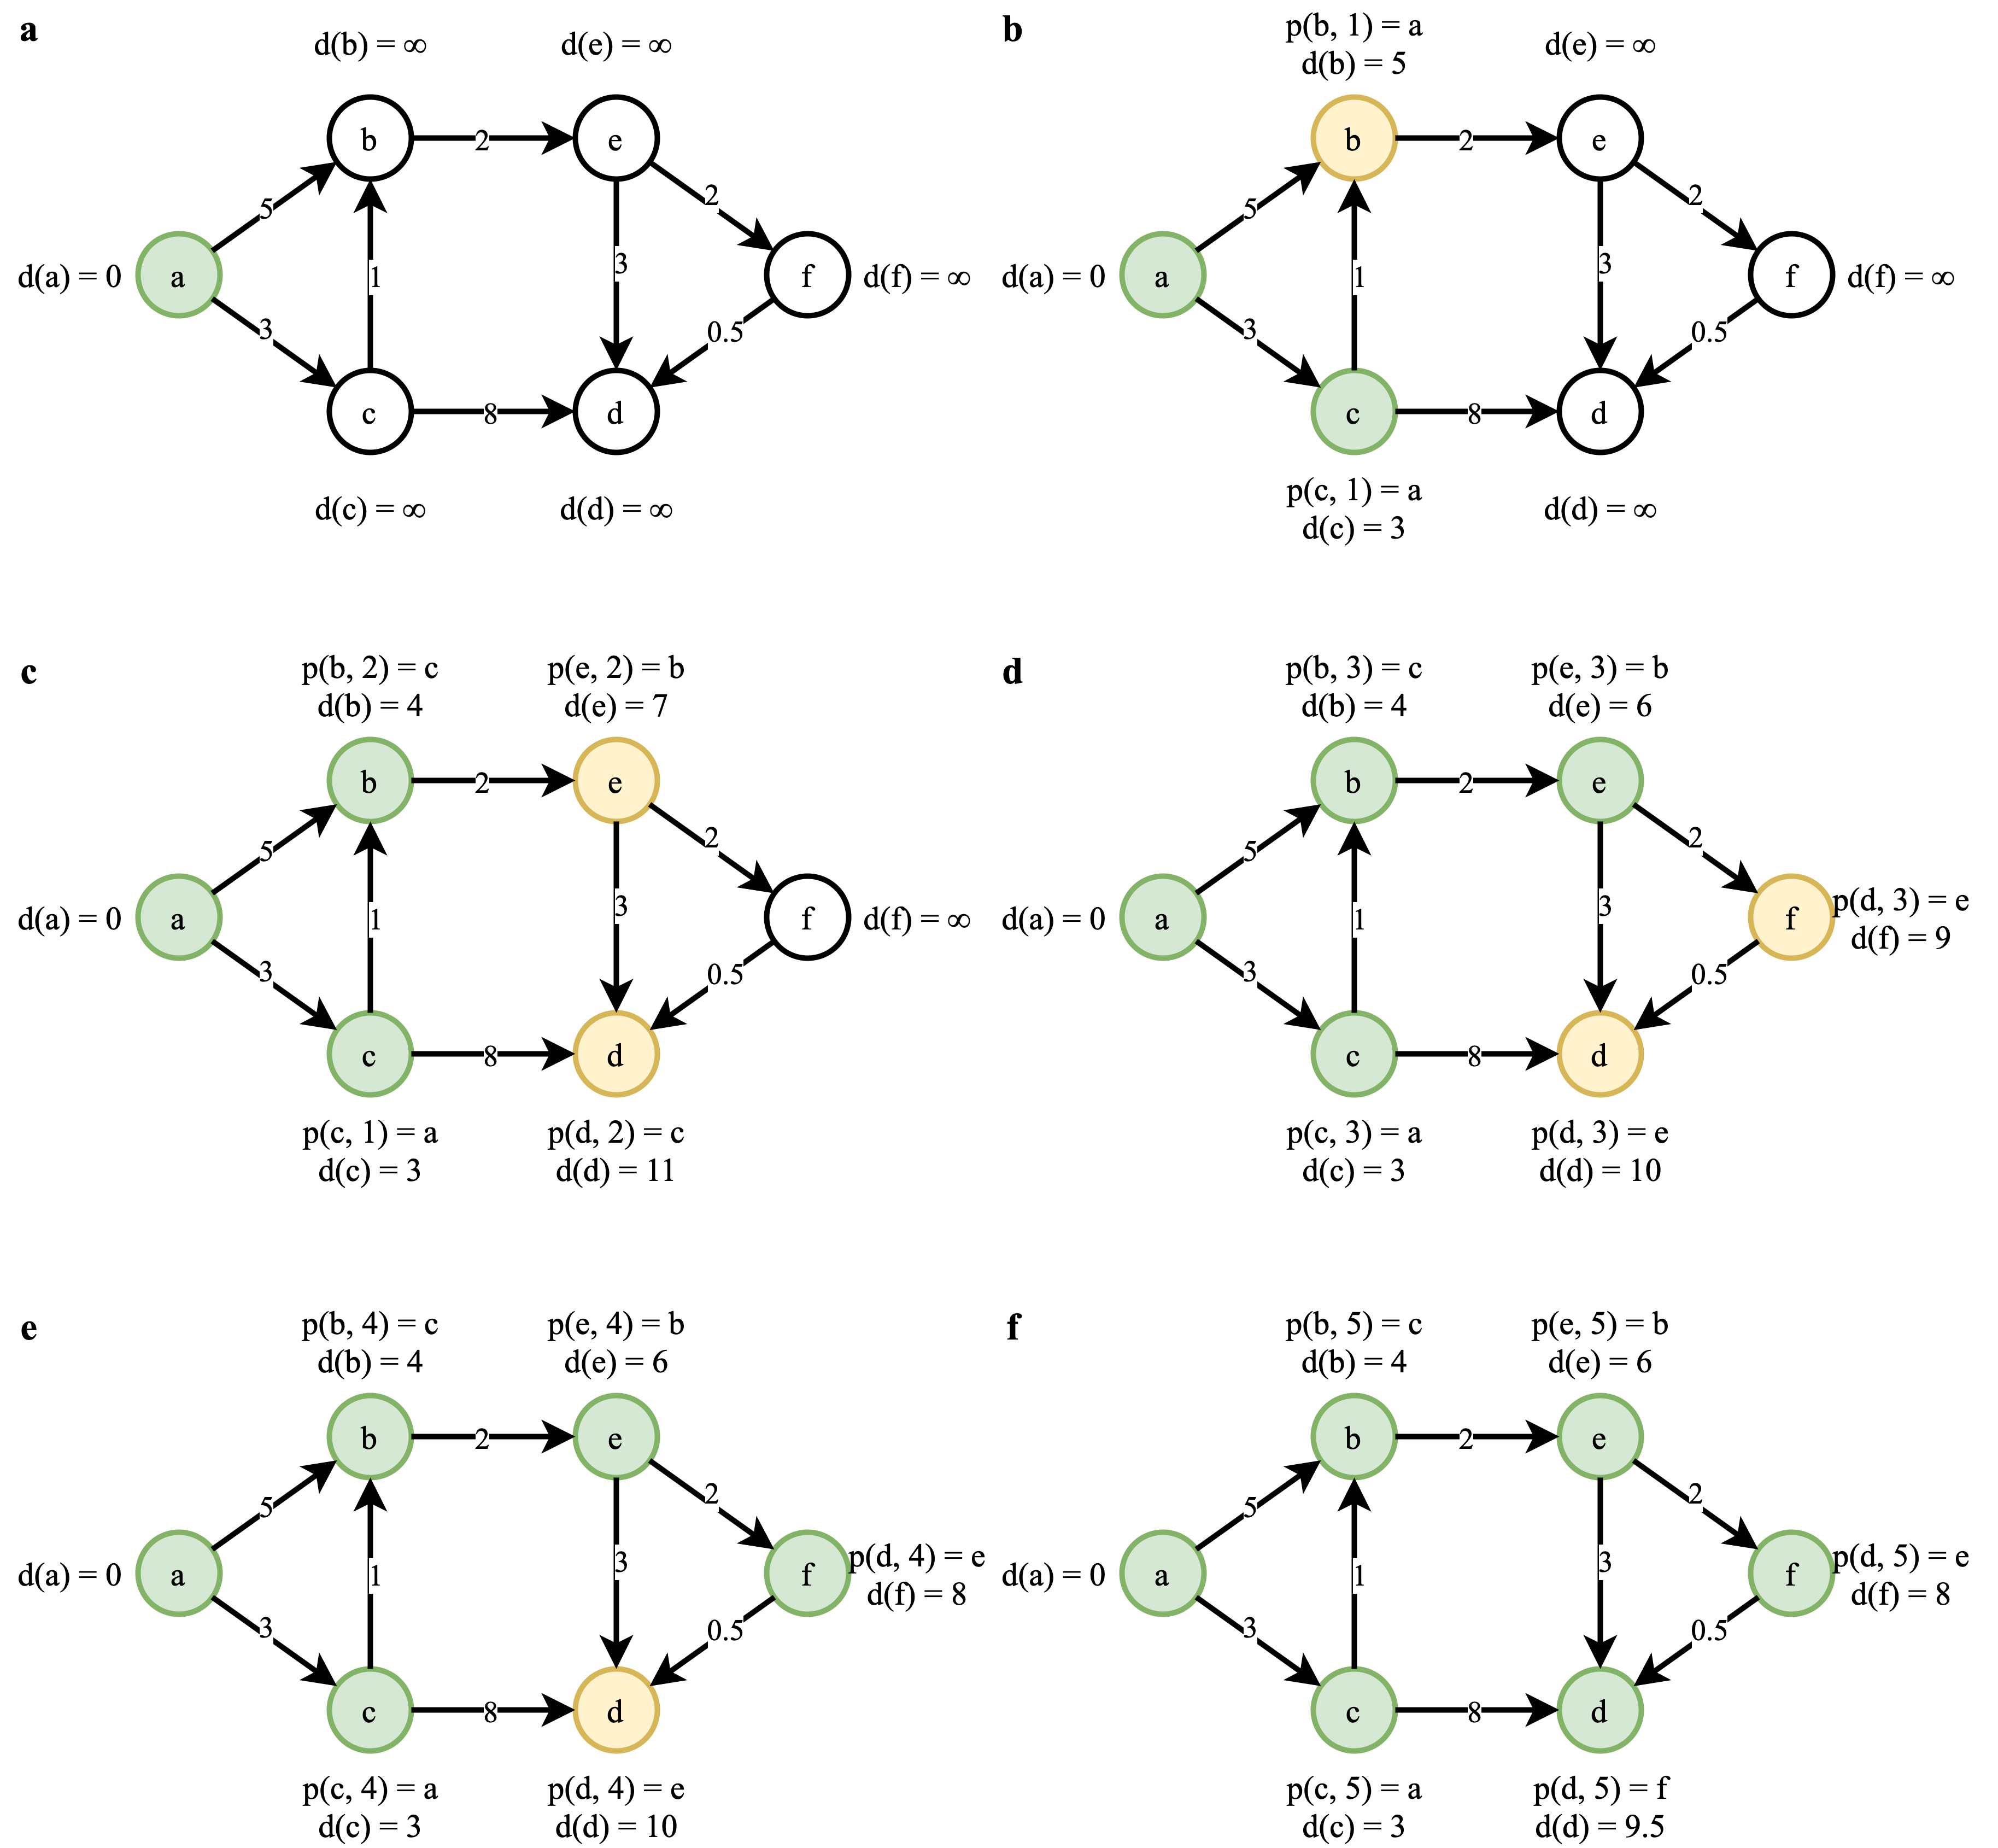
\includegraphics[width=1\textwidth]{./figures/ch3-bf.png}}
\caption{贝尔曼-福特算法示意图}
\label{fig-ch3-bf}
\end{figure}

贝尔曼-福特算法和迪杰斯特拉算法在结构上非常相似 \cite{BFOPTI} 。迪杰斯特拉算法只查看每个节点的直连邻居节点,而贝尔曼-福特算法在每次迭代中都会遍历每条边。贝尔曼-福特算法的时间复杂度为:最佳情况下复杂度为$O(E)$;平均情况下复杂度$O(|V||E|)$;最坏情况下复杂度也是$O(|V||E|)$。空间复杂度为$O(V)$。贝尔曼-福特算法经常应用用于计算路由算法中的最短路径或者寻找最短路径,因此是非常适合用于本文对段路由航点计算的场景的。

2. 段列表生成算法

在计算了辅助图中每条链路的权重后,段列表生成算法将计算出尽力满足请求流量延迟要求的完整段路由标签列表。首先描述一下问题,假设网络中的所有节点都是段路由节点,并可能成为请求流量到达的段路由域的第一节点$s$或目的节点$t$。当前有一条流量的源节点和目的节点分别为$s$和$t$,并且需要有一个小于$d_{target}$的延迟。段列表生成算需要在网络存在动态流量的场景下构建段路由标签列表,使得通过这组段列表进行调度的流量有较大的可能实现端到端的时延尽量小,以至于时延小于目标值$d_{target}$。

贝尔曼-福特算法是基于松弛原理的。在每一步的计算中,最优权重路径逐渐被一个较小的新值所取代,直到最后达到最优解。从源节点到目的节点的非环形可达路径在图中最多有$|V|-1$边。贝尔曼-福特算法松弛了所有的链接,所以这个过程需要重复$|V|-1$次。该算法允许通过限制跳数来确定贝尔曼-福特算法是否需要继续。在每次迭代中,该算法将从源节点到目的节点的长度为$x+1$的路径的权重与上一次迭代中长度为$x$的路径的权重进行比较,并记录权重小于两者的路径。并更新最优路径。逐渐放宽路径长度,将得到从给定的源节点到目的节点的最优加权路径。

\subsection{算法时间复杂度分析}

在上述算法中,计算链路中心度的时间复杂度为$O(|V|log|V|+|E|)$,其中$k$为考虑的前$k$路径,$|V|$为节点数,$|E|$为边的数量。链接到达率和链接拥塞度可以直接采集或者通过时间复杂度为$O(1)$的方法计算得到,因此推导链接权重的时间复杂度可视为$O(|V|log|V|+|E|)$。计算辅助图的时间复杂度为$O({|V|}^{3/\alpha})$。然而,这两者都是由网络变化事件或定时器驱动的,因此在考虑段列表生成的时间复杂度时可以忽略。

基于贝尔曼-福特算法计算段路由列表的算法的时间复杂度为$O({|V|}^{3/\alpha})$,由于存在仅由${|V|}^\alpha$的节点组成的辅助图,因此时间复杂度降低。

\section{本章小结}

在本章设计了一种参考链路时延构建链路权重选择段路由段列表的算法。该算法从多个角度测量并分析数据特性和研究的模型需求构成链路权重计算公式,通过对集中网络节点介数中心度进行分析得出用更少节点构建辅助图的拓扑降维方案,并使用贝尔曼-福特算法来推导计算出段列表。

本章的算法仍有一些不足之处,例如,链路到达率是一个相当理想的值,在现实的网络中可能很难使用。此外,带内遥测的准确性会影响算法的结果,目前在商业交换机中,带内遥测数据是每3秒或10秒收集一次。因此,未来的工作是研究如何在算法中有效地收集和计算每个参数,并在物理网络中验证该算法。

\chapter{基于差分时延分组的分布式路径选择算法}

\section{引言}

在上一章提出的算法中,集中式的段路由路径选择算法具有全局调优,资源协调整合的优点,但是在面对网络流量动态变化频繁,对服务质量的实效性要求较强的的时候,集中式的控制计算方式就会产生较大的处理延迟,因此本章将从分布式的角度对段路由的时延需求进行保障。

除了计算时延需求的段路由航点的分布式优化外,上一章提出的算法只能尽力保障业务流量的时延更低,但是对于业务提出的明确时延需求并没有针对地进行资源分配,这主要是因为时延的资源计算更为复杂,无法像计算剩余带宽一样直接减去使用带宽,并且先到先服务的尽力而为架构在一定程度上也是可以保障互联网的公平性。但是对于需要差分服务质量的网络,这种方案就不太可行。因此为了对时延服务质量需求进行更有针对性的资源分配,本章将用对时延进行差分分组的方式设计分布式保障时延需求的算法。

本章将对基于时延的路径选择算法进行建模分析、算法阐释,并给出实验验证结果。本文参考边界网关协议的实现逻辑,考虑在航点之间如何进行数据交互以及使用怎样的分布式算法可以计算得到具有最好的时延保障效果的段路由航点列表。与第三章侧重点的不同主要在于,第三章的算法是控制器运行的算法,而第四章的算法主要是数据面分布式的协议和算法。

\section{问题模型}

在广域网的路由系统中,按照规划或地域原因往往被分为很多的 \gls*{AS} ,自治域内部使用内部网关协议进行内部通信,自治域之间使用边界网关协议进行跨域通信,整个网络中的网元节点要运行内部网关协议、边界网关协议等路由协议来保证网络内部节点的互相连通性,这些协议也会随着网络动态变化实时更新网络交换机的路由信息表,多种类型的路由表信息经过一定的算法整合就将生成 \gls*{FIB} ,当交换机收到一个新的数据包时,它会直接通过查找转发信息库将数据包转发到正确的端口,最终实现全网路由可达。当段路由运行在广域网中时,广域网的路由系统会被类似地划分为很多的分段路由域用于对标签进行管理,通常也不要求所有网元节点都支持段路由功能,而是部分节点具有封装、传递、弹出段路由报文头的功能即可,如图4-1所示。因此这些具有段路由功能的网元节点实际上组成了一张节点数和链路数更少的段路由网络。

\begin{figure}[htbp]
\setlength{\abovecaptionskip}{15pt plus 3pt minus 2pt}
\centerline{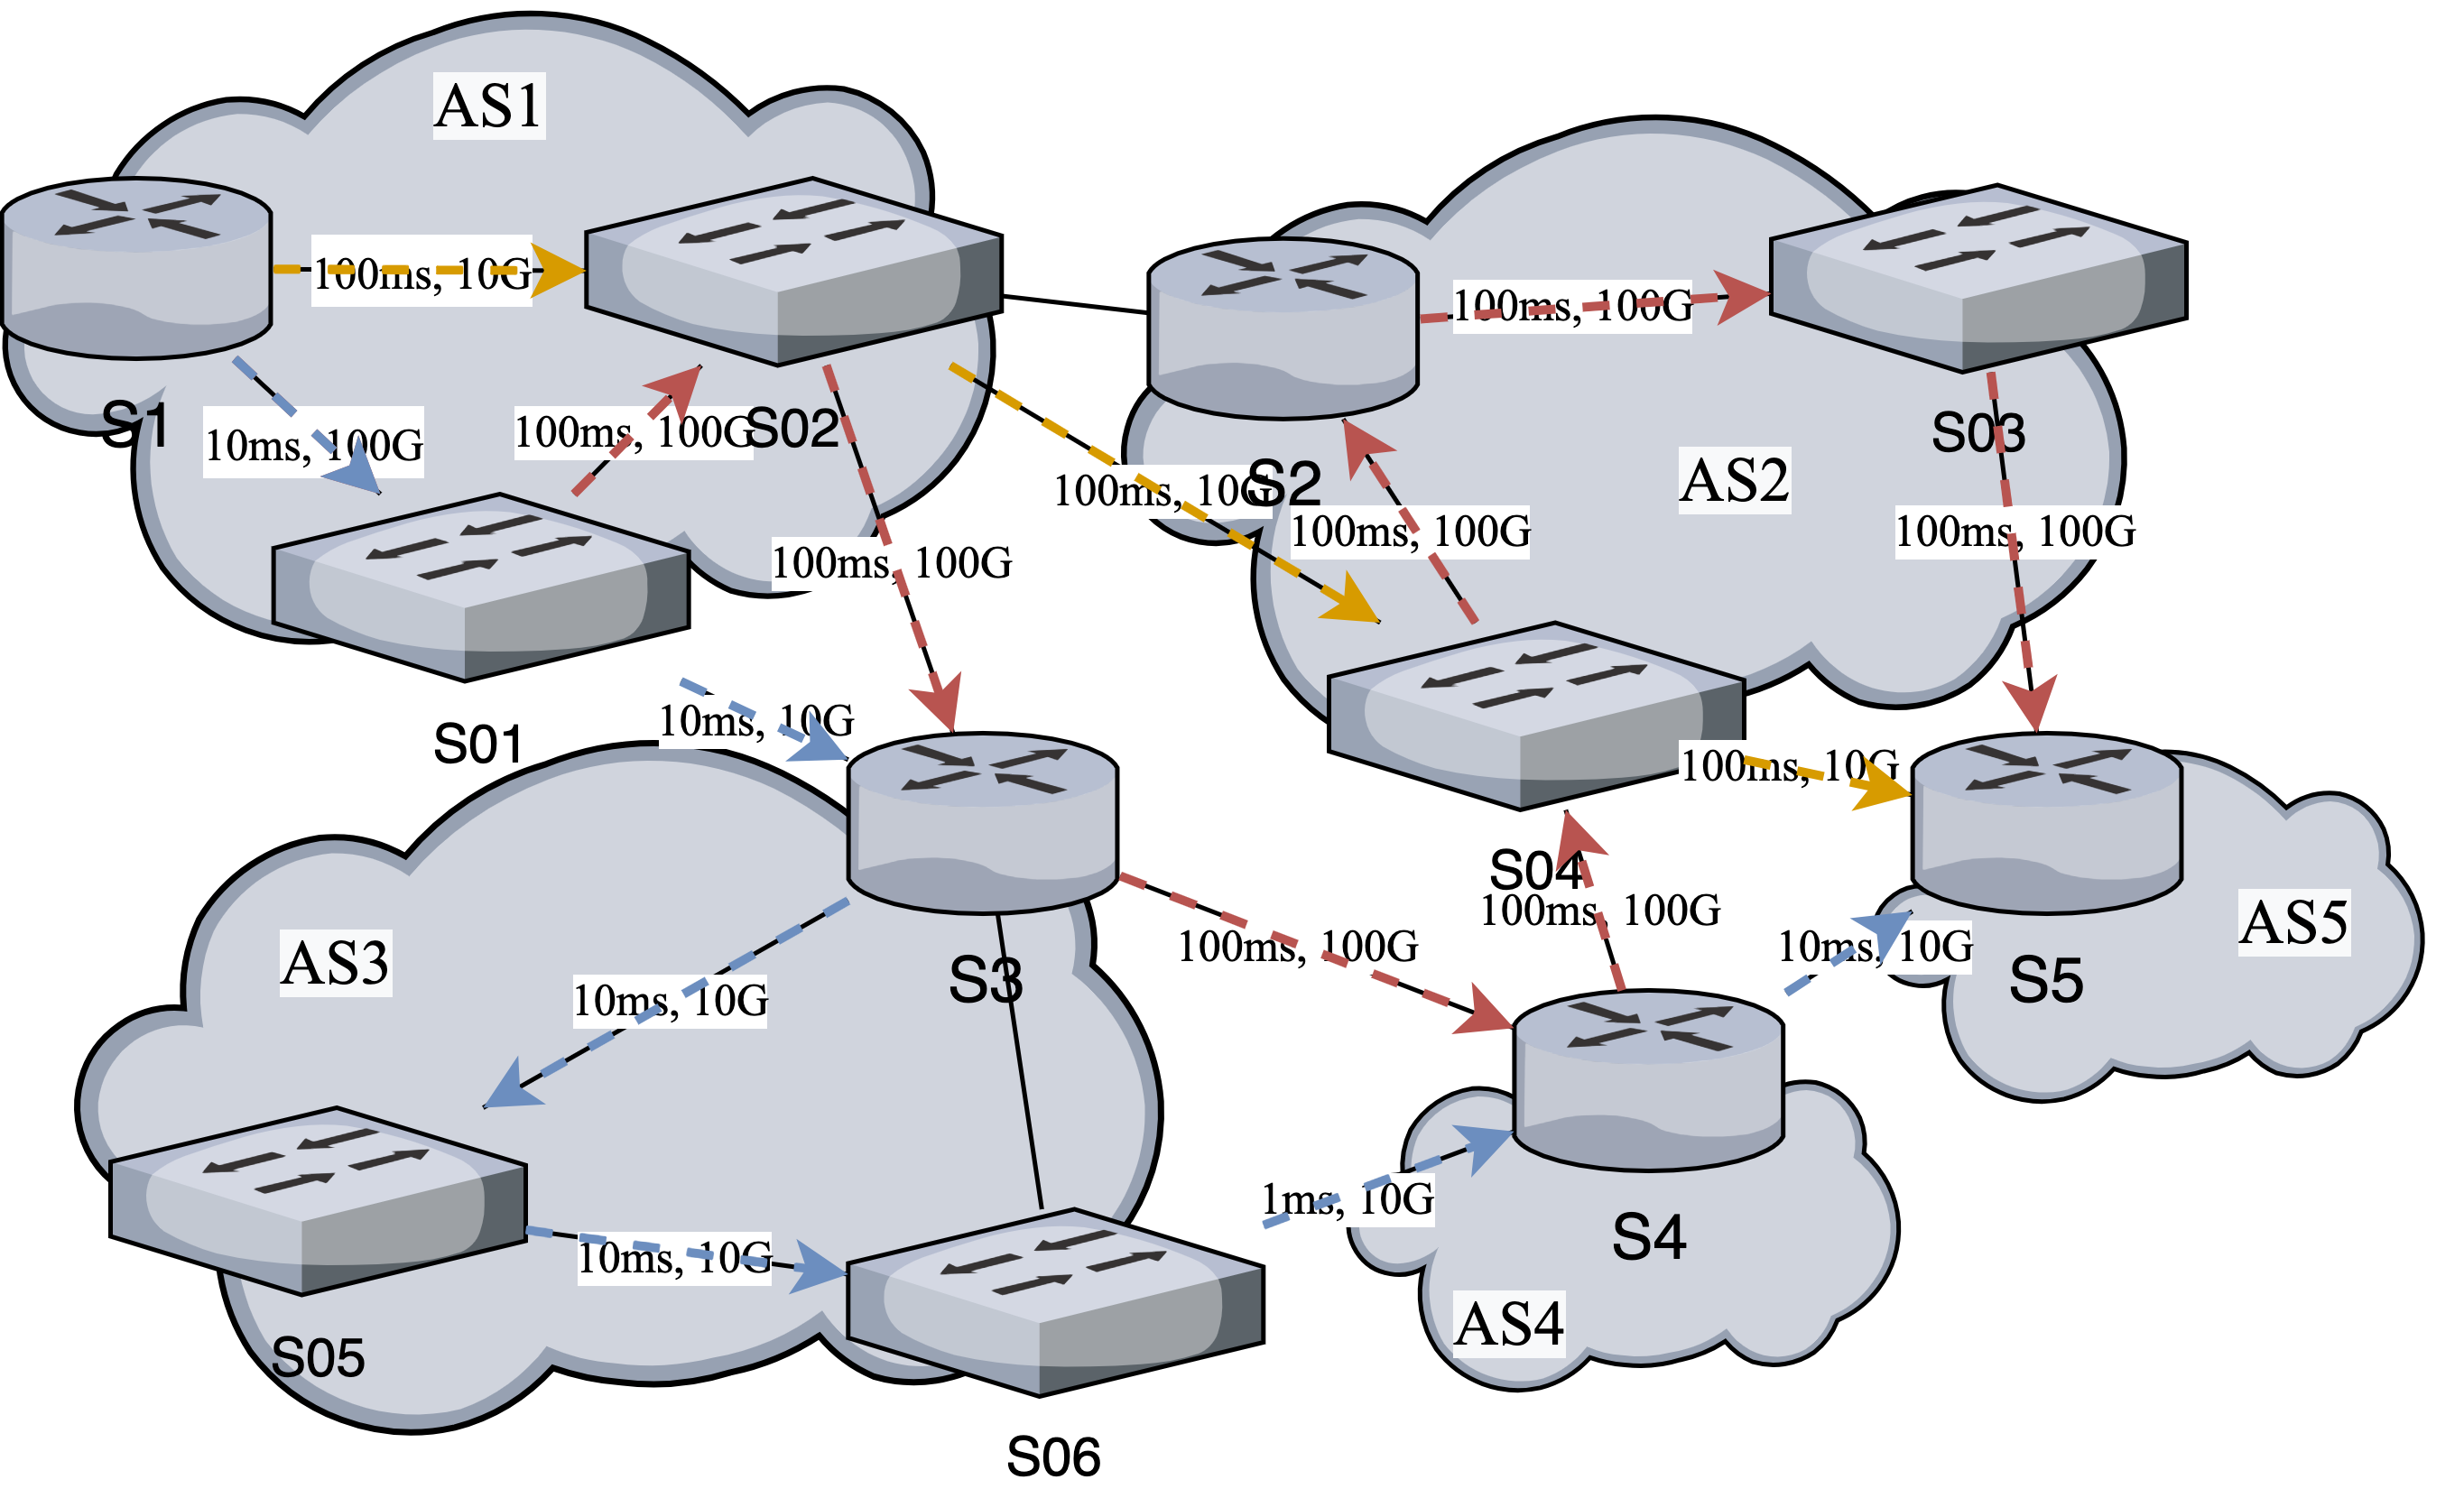
\includegraphics[width=1\textwidth]{./figures/ch4-problem-model.png}}
\caption{分布式段路由选路方案示意图}
\label{fig-ch4-problem-model}
\end{figure}    

端到端报文在到达某个段路由交换机时是从一个段路由域内去往另一个段路由域,并且携带一个目标时延,入口段路由节点就会按照本地的段路由策略选择合适的段路由标签列表,并封装到报文头部指导转发路径。假设段路由策略被配置为按照最短跳数选择路径。如图4-1所示,则在AS1中,目的地址在AS5中的数据包都将沿着图中黄色路径(AS1(S1 -> S02) -> AS2(S04) -> AS5(S5))转发;如果按照带宽选择路径,目的地址在AS5中的数据包都将沿着图中红色路径(AS1(S1 -> S01 -> S02) -> AS3(S3) -> AS4(S4) -> AS2(S04 -> S2 -> S03) -> AS5(S5))转发;而如果按照时延选择路径,目的地址在AS5中的数据包都将沿着图中蓝色路径(AS1(S1 -> S01) -> AS3(S3 -> S05 -> S06) -> AS4(S4) -> AS5(S5))转发。

因此将网络拓扑图抽象为以全部网络节点为点集合,以全部链路为双向有向链路边集合的有向图,将适配流量所需时延作为优化目标构建数学模型,待求解对象为段路由节点内对其他节点进行时延表达的数据结构以及匹配目标时延的方法。用公式表达如下:

\begin{equation} \label{distributed segment routing target}
    min(\frac{|D_{target}-D_{redult}|}{D_{target}})
\end{equation}

\section{基于差分时延分组的分布式路径选择算法}

\subsection{算法概述}

差分时延的路径选择算法是一个分布式算法,任何段路由节点都需要参与其中。在差分时延的路径选择算法中,每个段路由节点内部维护一个差分时延段路由策略表,并通过ICMP协议获取本段路由节点到其余段路由节点的由传统路由系统计算得出的的默认路径的时延,记录这个时延是有意义的,因为当数据包从一个航点到下一个航点,一定是通过传统的基础分布式路由算法得到的选路结果。这些段路由节点间的时延将被类似边界网关协议宣告的方式传达给其他段路由节点,每个段路由节点将收到的消息更新在自己的差分时延段路由策略表。这部分算法和差分时延段路由策略表的数据结构将在4.3.4进行详细梳理。当这些测量结果在全网的段路由节点处整合收敛,网络中就形成了分布式的段路由节点优选差分时延矩阵。矩阵的规划和数据属性将在4.3.2进行分析。因此各个段路由节点就可以利用这些测量结果找到一对段路由节点之间的多条可达路径,且具有段路由节点之间路径的时延信息,即差分时延矩阵。在多条可达路径中,存在各种差分分组的时延,如1ms-10ms级、10ms-100ms级、100ms-1s级、1s-10s级等,这些时延信息将被段路由节点以时延矩阵的方式进行分类。当服务流量到达一个段路由节点的时候,就将对待服务流量的需求时延落入分级的差分分组中,并使用组内的段路由实现方案进行递归路径选择,并最终生成段路由航点列表,选择的结果将基于流量的五元组哈希和段路由方案的惩罚值,这部分内容将在4.3.5段路由航点列表生成算法中进行分析,本节算法思路的结构索引如图4-2所示。

\begin{figure}[htbp]
\setlength{\abovecaptionskip}{15pt plus 3pt minus 2pt}
\centerline{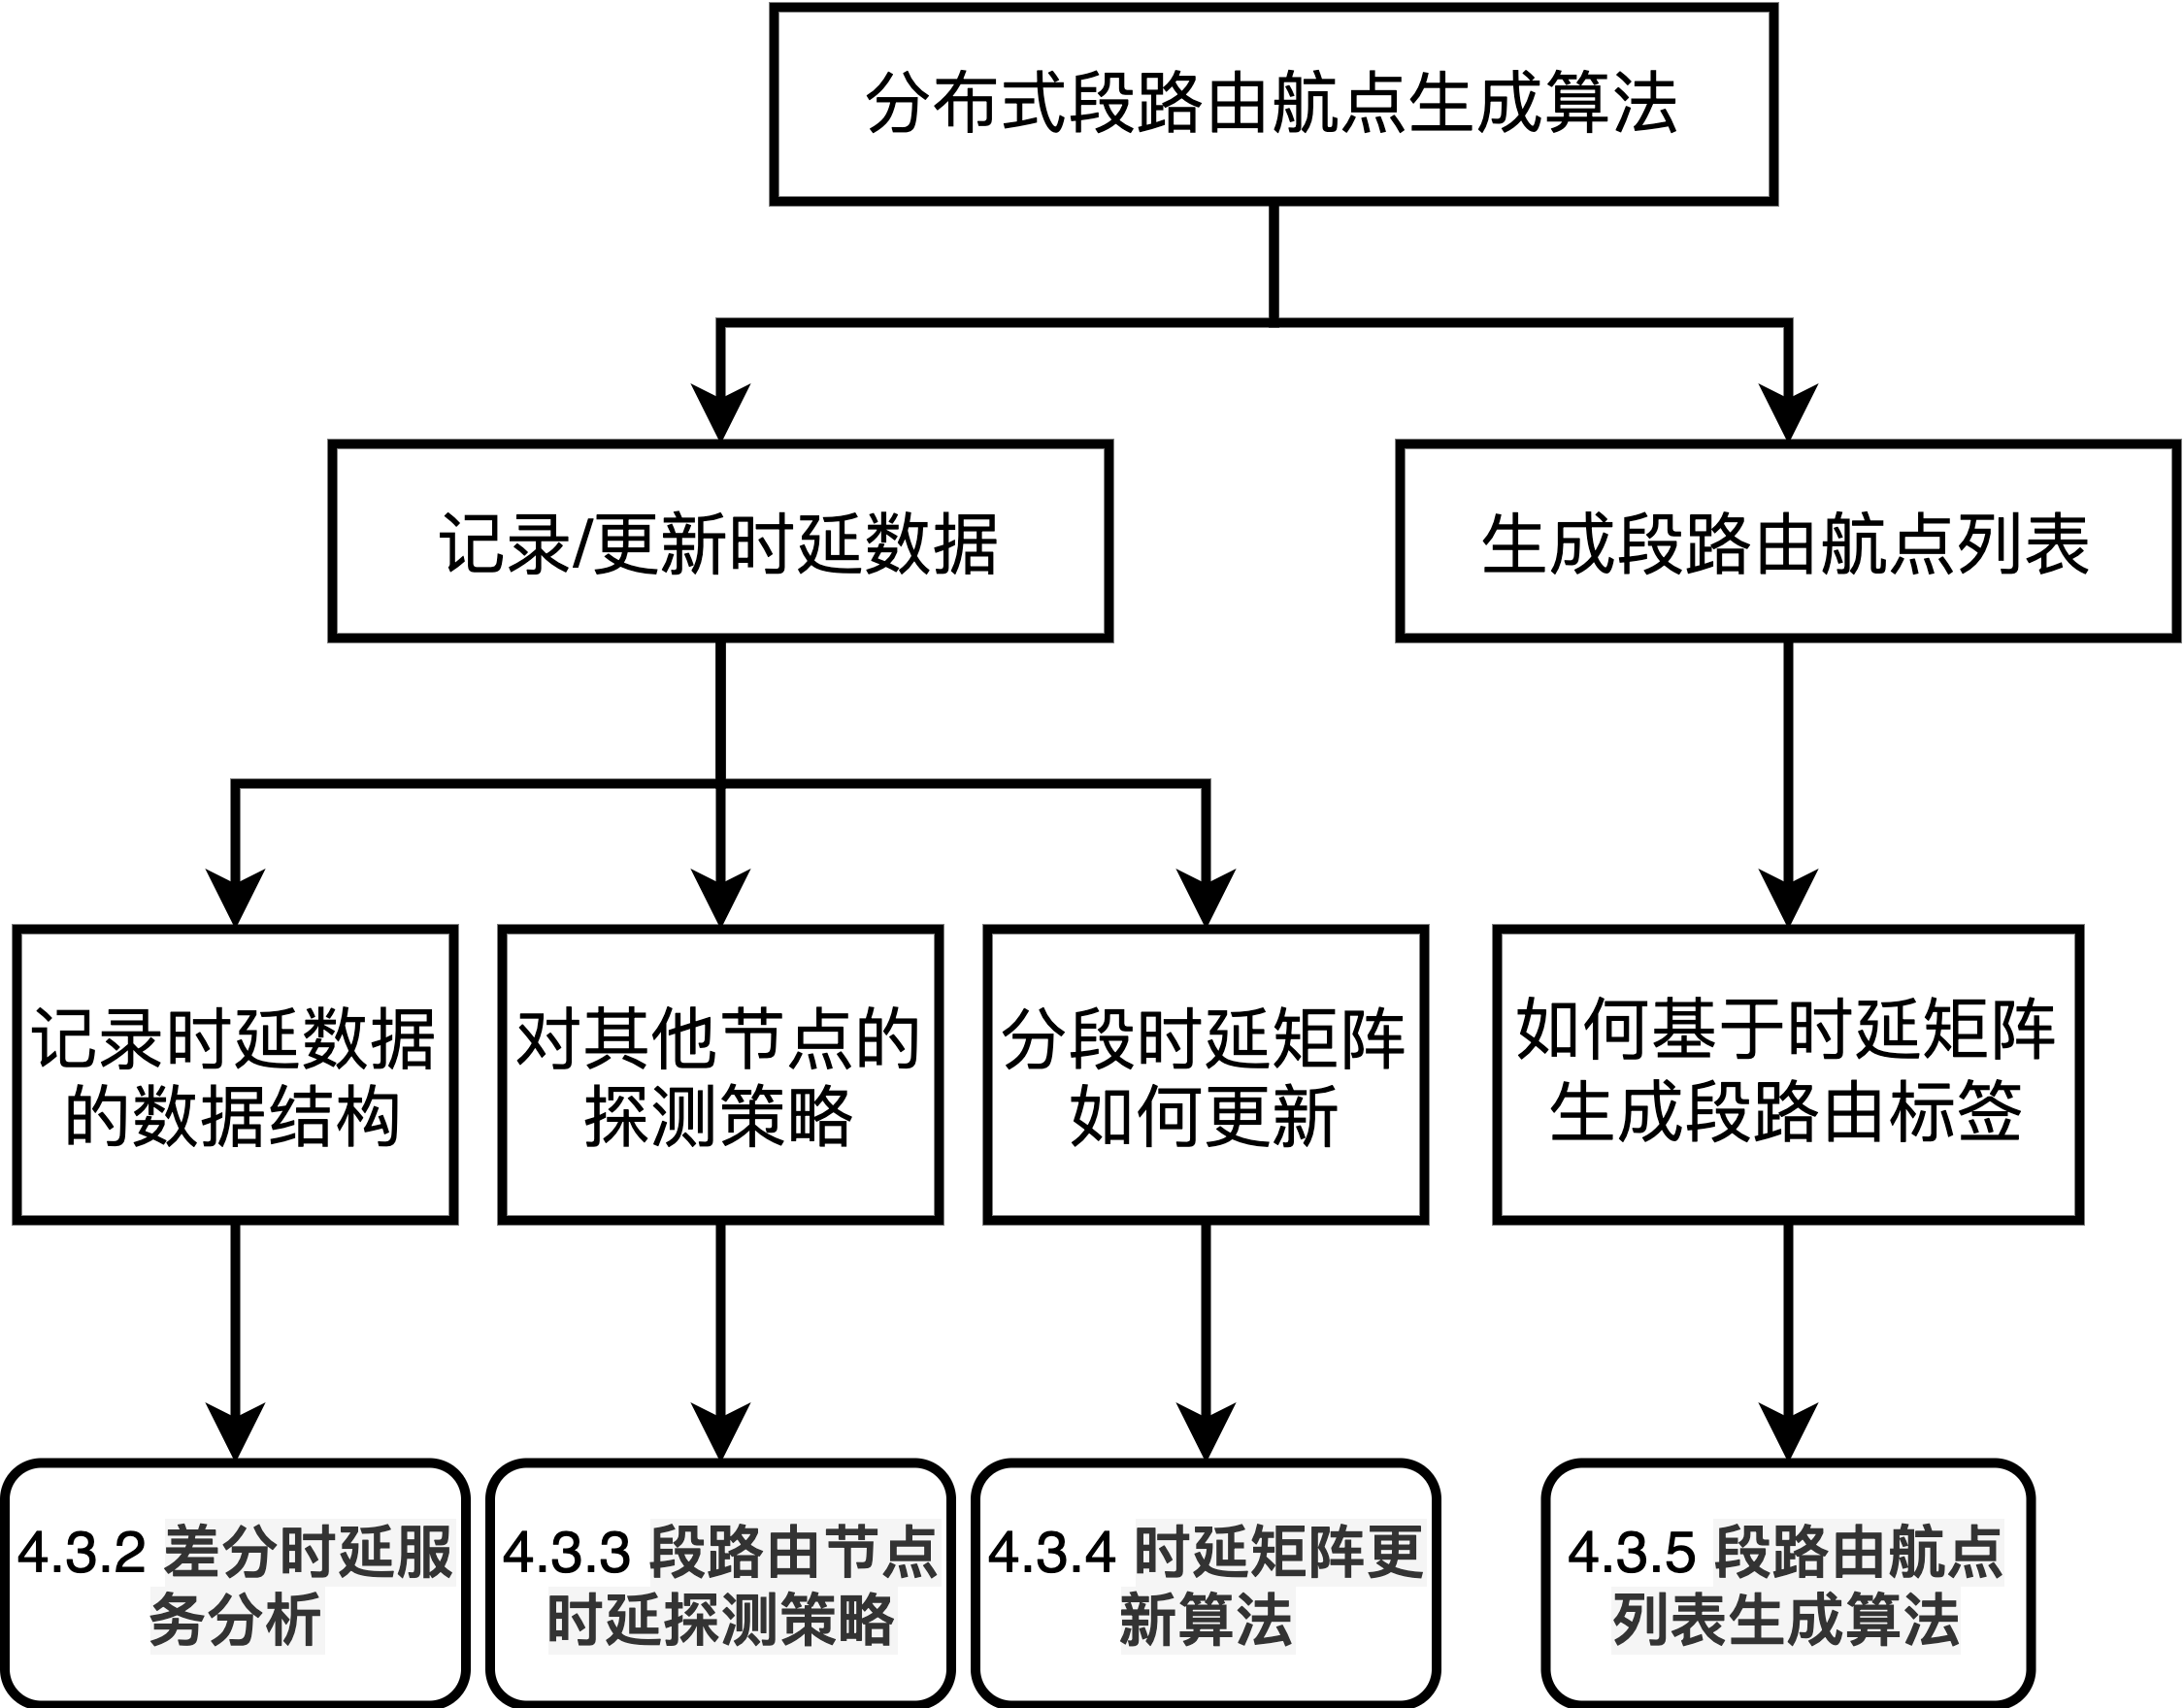
\includegraphics[width=0.8\textwidth]{./figures/ch4-ark.png}}
\caption{分布式段路由航点列表生成算法思路索引结构图}
\label{fig-ch4-ark}
\end{figure}

本章的算法主要有以下几个挑战:

\begin{itemize}
\item 挑战1:对于每一台交换机,时延探测的对象有谁?该挑战需要明确时延探测对象是因为如果选择探测全体其他段路由节点会造成过大的探测流量影响网络的吞吐,而过小的探测对象数目可能导致探测结果的不全面,无法得到时延最短的路径。
\item 挑战2:每个交换机需要以怎样的数据结构存储与其他段路由之间的时延信息可以做到占用较少的资源实现较高的效率?这是由于对于每一台运行路径选择算法的交换机都需要维护一张与其他组交换机间时延的表,段路由节点过多和时延分组的过多会导致表格以乘法关系的增长,这会造成比较大的数据冗余,因此需要设计更为合理的存储段路由节点间时延信息的数据结构。
\item 挑战3:怎样的时延矩阵更新方式可以更好得保障时延信息的及时性并且破坏稳定性?这个挑战的存在是由于类似路由翻滚的情况也有可能发生在段路由航点列表的算法结果选择上,本章希望可以得到一个抑制无效段路由航点列表计算结果翻滚的方案来降低相同时延需求和源、目的地址流量计算出的段路由列表方案来回切换的可能。
\end{itemize}

\subsection{差分时延分组分析}

段路由节点之间的时延根据段路由节点的地理位置会出现很大的差异,例如从国内一个可用区的数据中心中的两个段路由节点之间测量时延,大概仅有1毫秒的时延,这是因为同一数据中心由于其风和水电统一规划、地理位置比较接近,光线行程较短,因此时延很低,一般对时延需求很高的业务也会部署在同一个可用区测数据中心中;如果测量国内两个可用区之间的不同段路由节点之间时延,其时延大致在10毫秒的量级;而如果从国内到国外的两个段路由节点之间测量时延,大概会到100毫秒左右。这是因为有研究认为互联网的往返时延即RTT随着互联网上数据分组从源节点到目的端经过的中转路由器的个数增加而增加,即往返时延与本文所定义的段路由通信跳数成正比。有一些研究表明链路两端距离小于5000千米的主要发生时延主要由排队时延组成,而链路两端距离大于5000千米的主要发生时延主要由传播时延组成 \cite{DELAY} 。综上所述,段路由节点之间的地理位置差异造成了彼此间通信的时延差异。

段路由节点会按照4.3.3描述的规则对其他段路由节点进行时延探测,时延探测结果被分成几类,每个段路由节点维护一个本节点到所有备选段路由节点组的时延记录数据结构,首先按照差分时延分段的机制,将目标时延分成几个区间,1毫秒到10毫秒,10毫秒到100毫秒,100毫秒到1秒…,在段路由节点中存储的数据结构如下表所示:

\begin{table}[]
\begin{tabular}{|p{0.2\textwidth}|p{0.7\textwidth}|}
\hline
1毫秒到10毫秒 & {[}SR目的节点1:\{下一跳SR节点组1, 总时延1\}, SR目的节点2:\{下一跳SR节点组2, 总时延2\}, ...{]} \\ \hline
10毫秒到100毫秒 & {[}SR目的节点3:\{下一跳SR节点组3, 总时延3\}, ...{]} \\ \hline
100毫秒到1秒 & {[}SR目的节点4:\{下一跳SR节点组4, 总时延4\}, ...{]} \\ \hline
... &  \\ \hline
\end{tabular}
\caption{节点时延矩阵结构图}
\label{table-delay-metric}
\end{table}

其中SR目的节点以哈希集合方式存储,目的节点对应的段路由方案列表用优先级队列存储,即队首时延最低,逐次递增。

\begin{figure}[htbp]
\setlength{\abovecaptionskip}{15pt plus 3pt minus 2pt}
\centerline{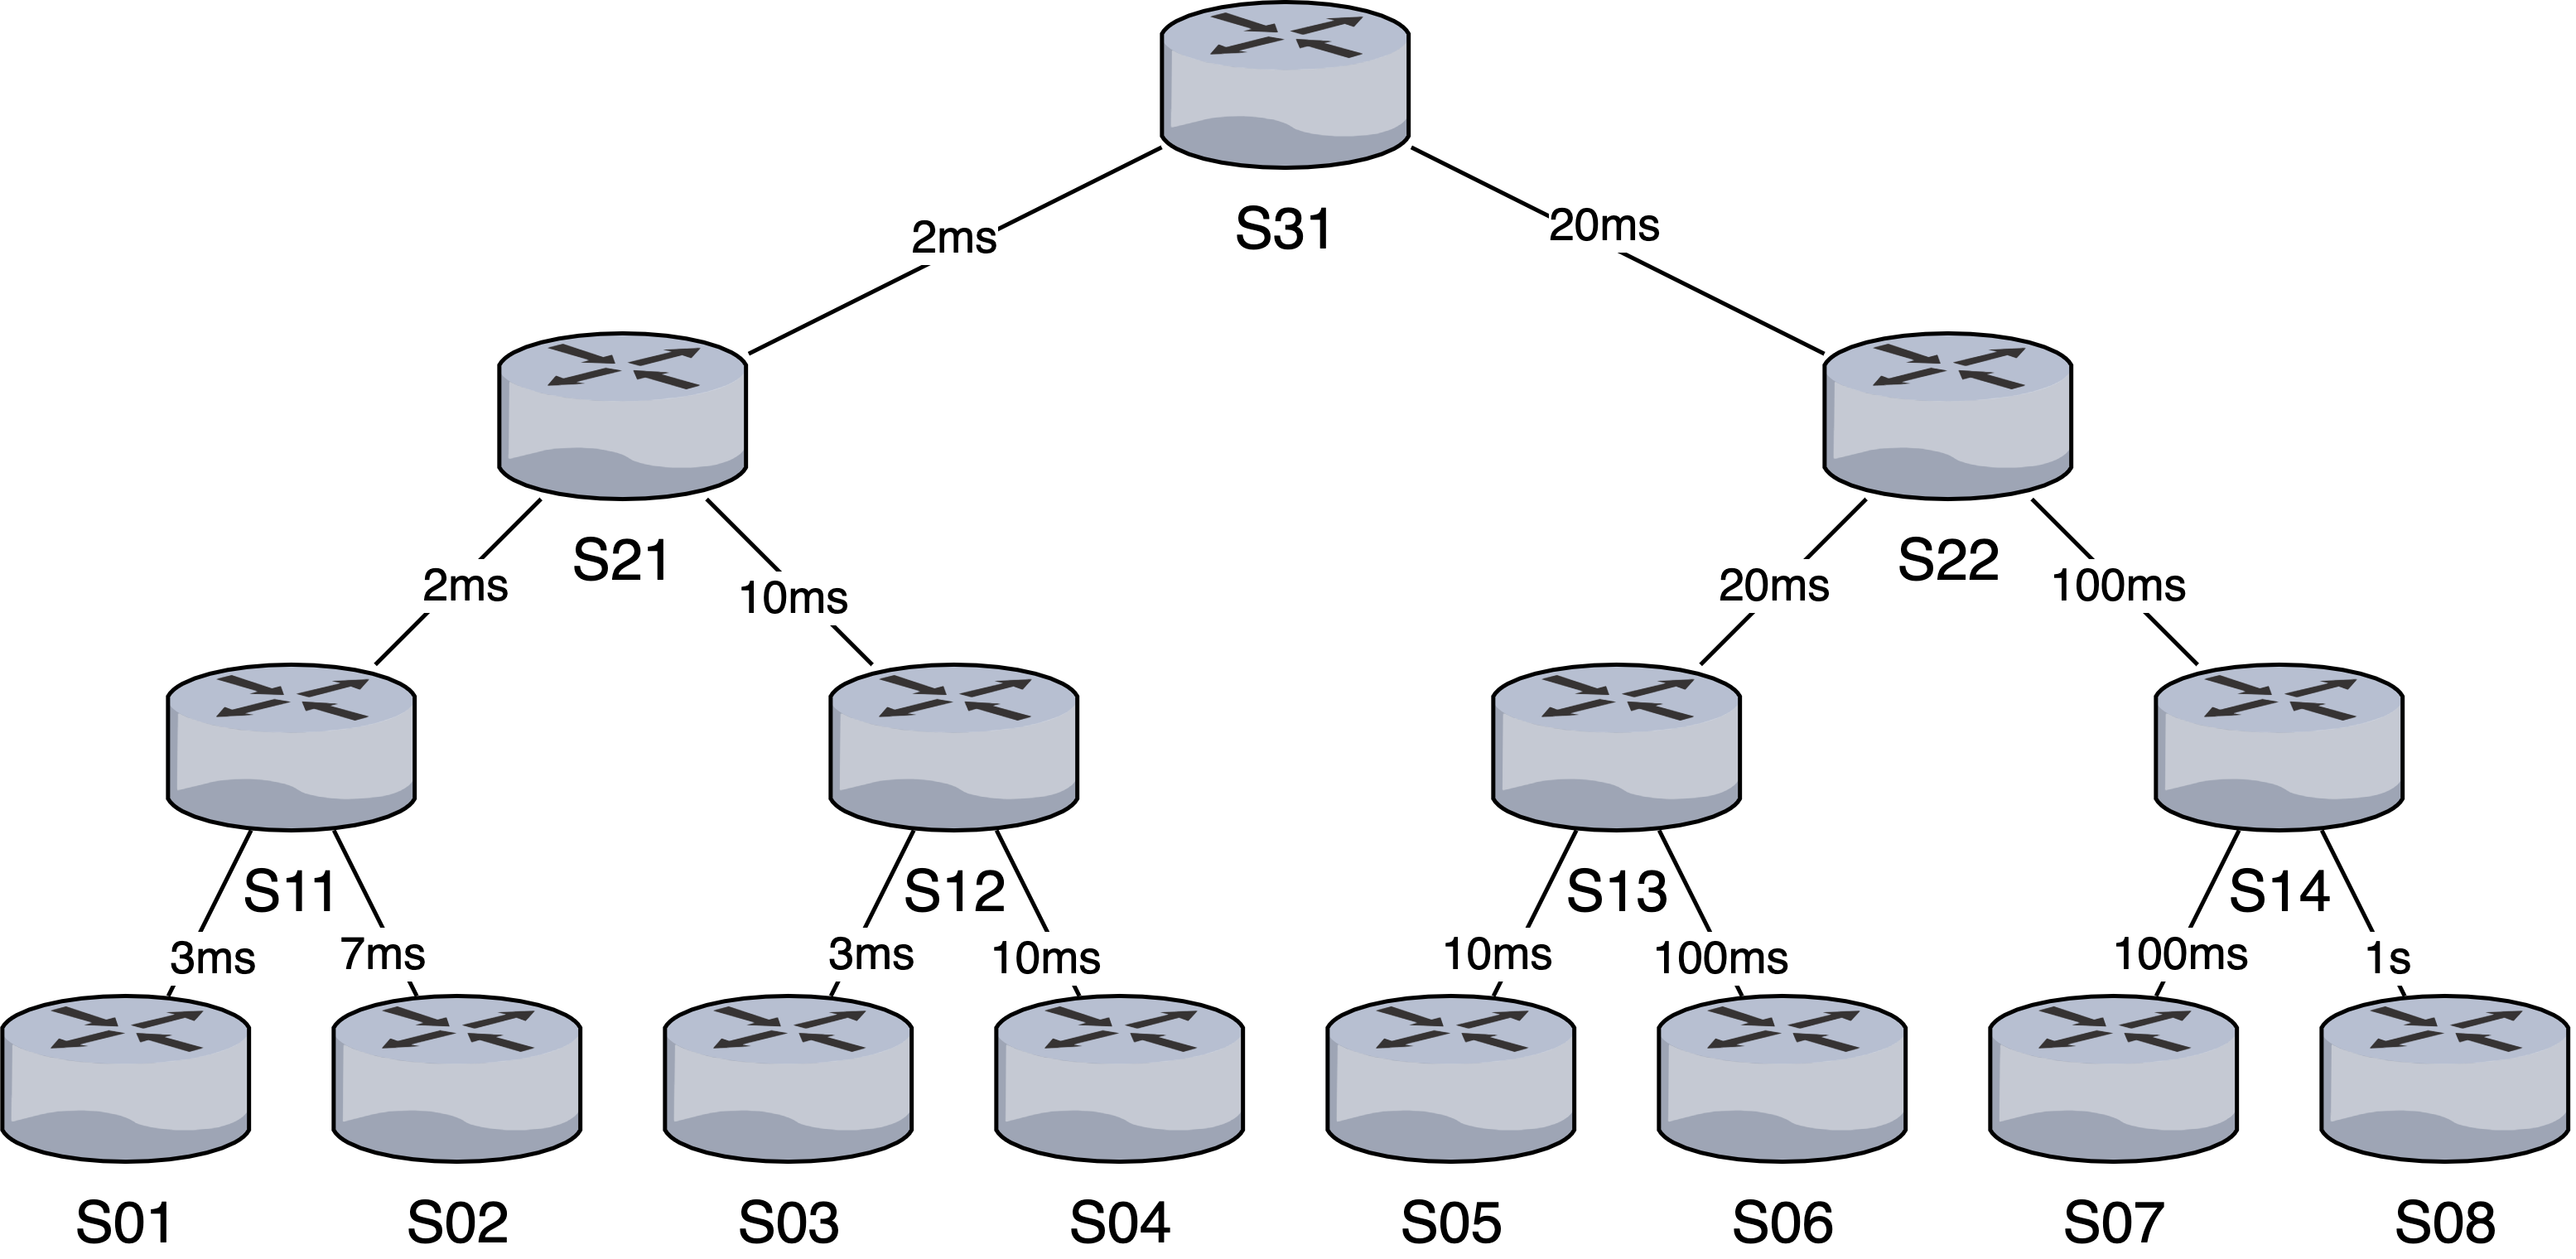
\includegraphics[width=0.8\textwidth]{./figures/ch4-tree-topo.png}}
\caption{段路由差分分组时延矩阵示意拓扑图}
\label{fig-ch4-tree-topo}
\end{figure}

以10毫秒到100毫秒的时延区间为例,如上图所示,$S_{31}$的段路由节点可以得到如下表的时延采集记录。

\begin{table}[htbp]
\begin{tabular}{|p{0.2\textwidth}|p{0.7\textwidth}|}
\hline
1毫秒到10毫秒 & {[}S21:\{nil, 2ms\}, S11:\{S21, 4ms\}{]} \\ \hline
10毫秒到100毫秒 & {[}S22:\{nil, 20ms\}, S12:\{S21, 12ms\}, S13:\{nil, 40ms\}{]} \\ \hline
100毫秒到1秒 & {[}S14:\{S22, 120ms\}{]} \\ \hline
\end{tabular}
\caption{节点时延矩阵填写示意图}
\label{table-fullin-delay-metric}
\end{table}

\subsection{段路由节点时延探测策略}

每个段路由节点在选择需要探测的节点列表时有一些潜在的问题。如果让每个节点探测所有其他节点就会造成高带宽开销的代价;而如果让每个节点随机探测一组节点就无法保证任何节点对的两个探测集的交集是非空的,即不能保证每个节点都被探测到。因此本节会提出一种可以较为公平探测段路由节点的算法,并且造成较小的带宽费用。

\begin{figure}[htbp]
\setlength{\abovecaptionskip}{15pt plus 3pt minus 2pt}
\centerline{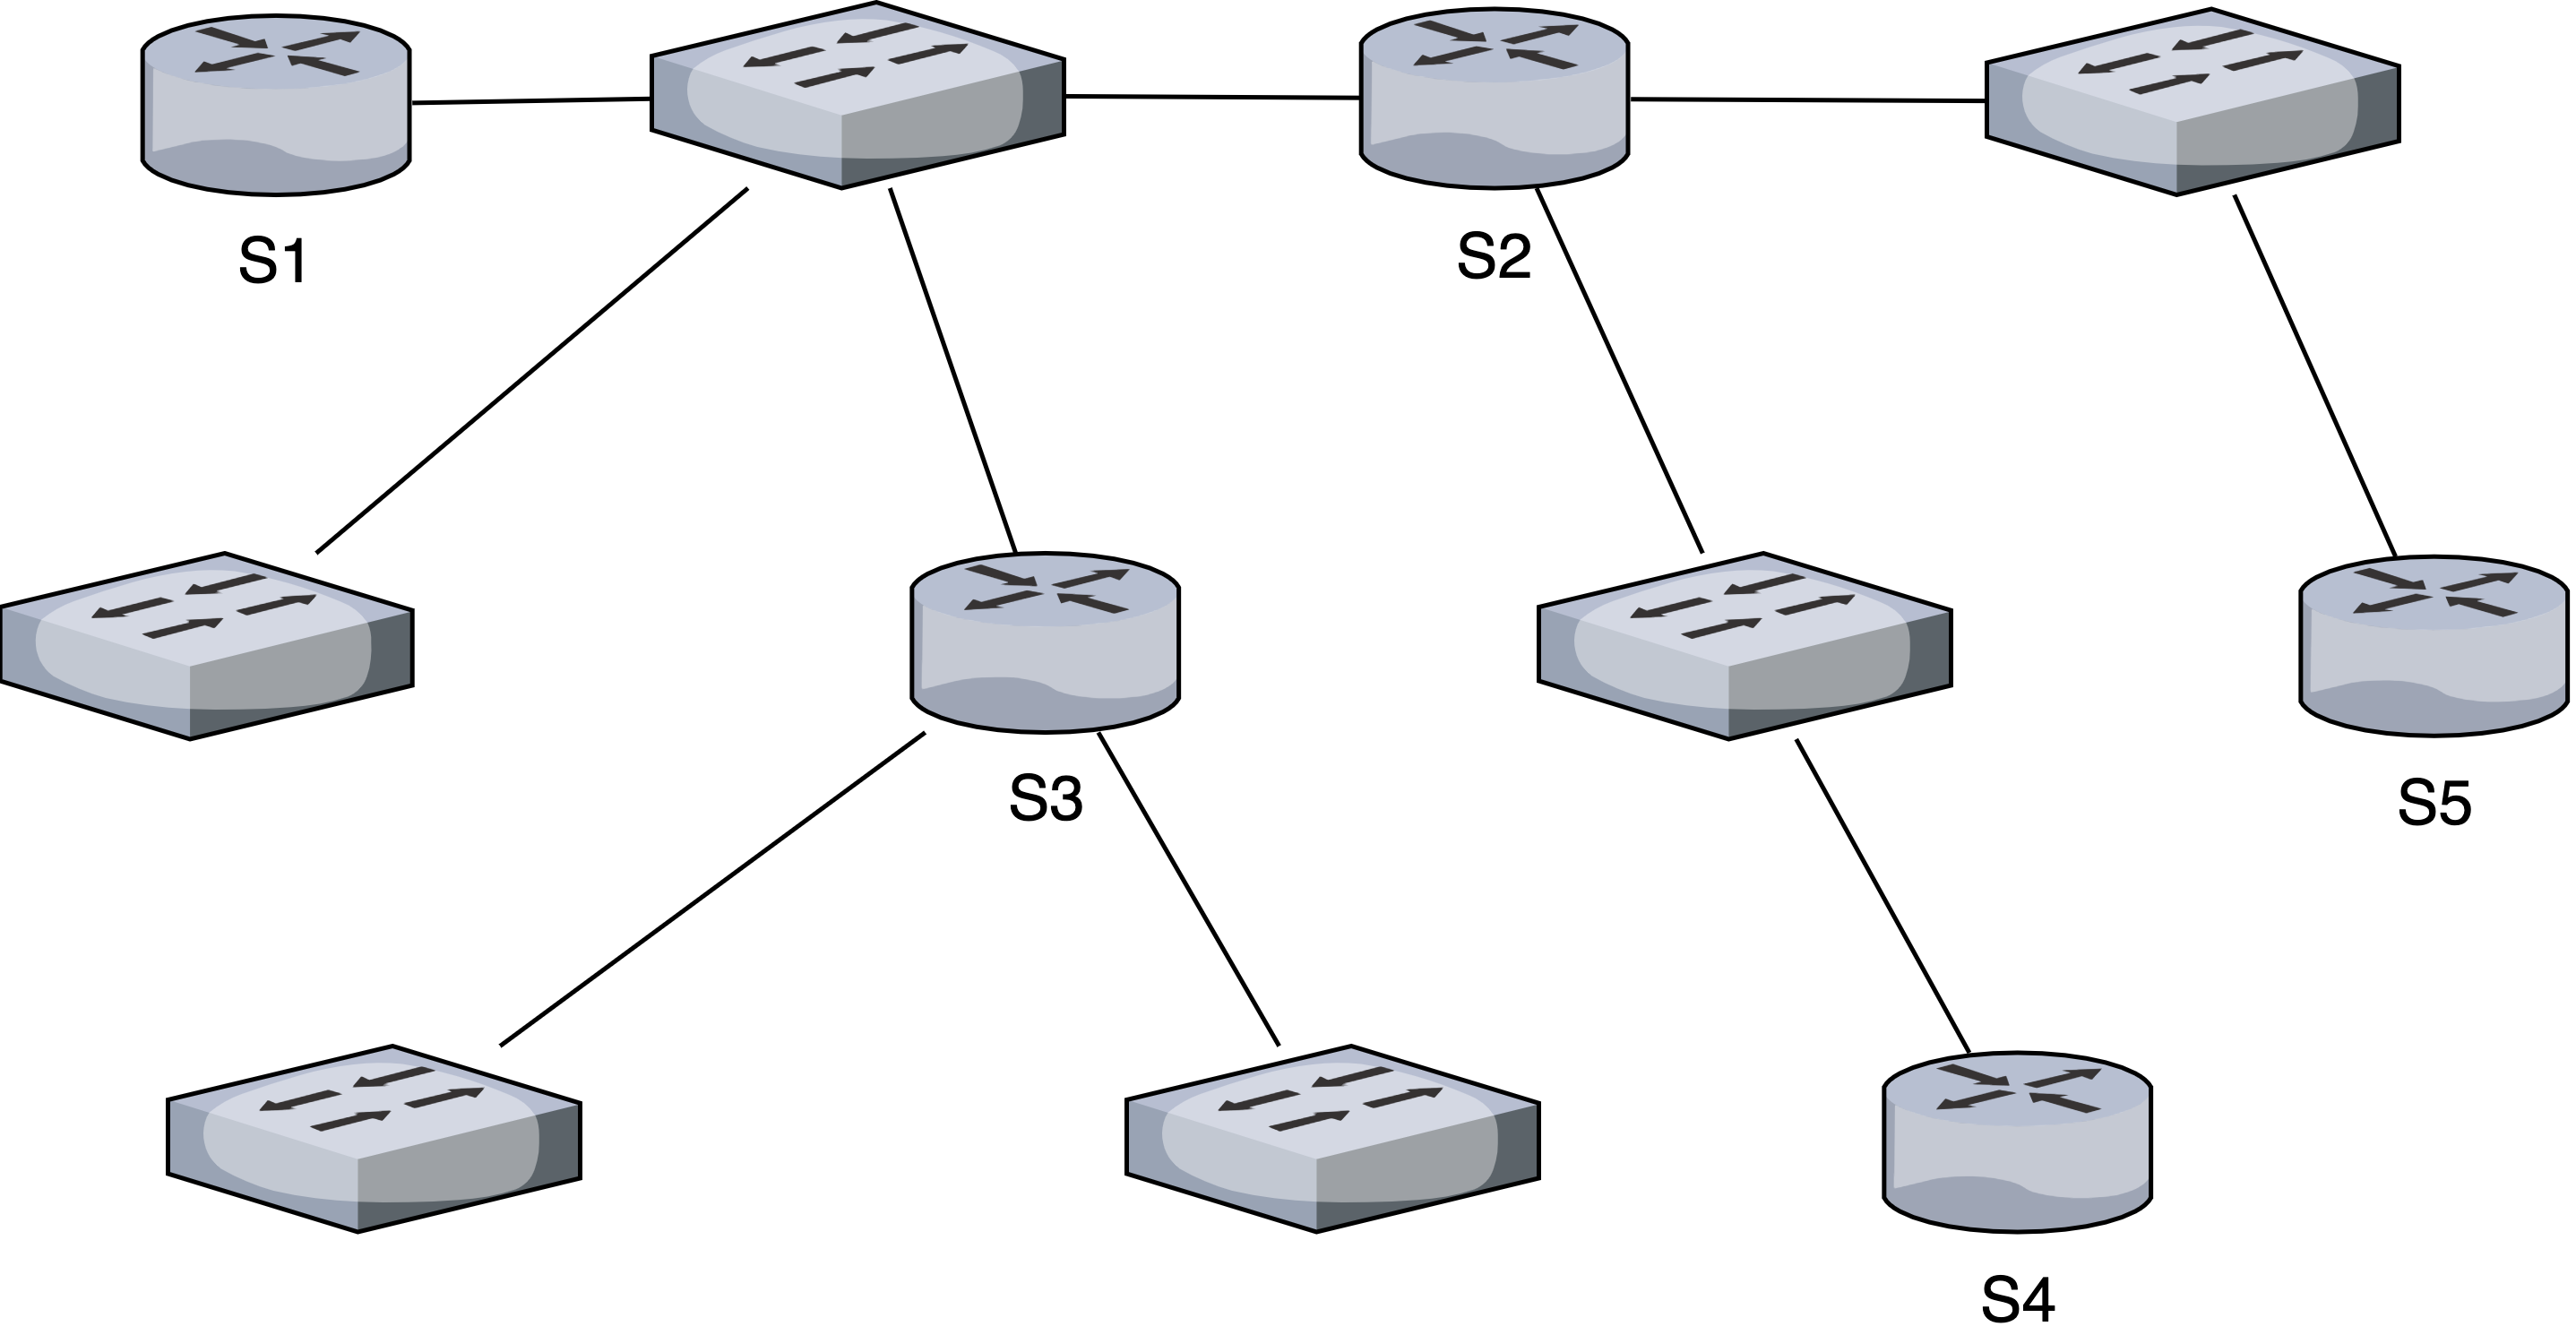
\includegraphics[width=0.7\textwidth]{./figures/ch4-random-topo.png}}
\caption{段路由节点探测列表生成策略拓扑示意图}
\label{fig-ch4-random-topo}
\end{figure}

首先从基于每个节点探测所有其他节点的方案开始展开,如果源段路由节点的报文被发送到另一个段路由节点,那么这个节点会返回一个回复报文来帮助源节点记录时延,由此可以得出一个判断,任何一个节点收到一个探测报文都会认为自己是源节点可达的段路由节点。但是为了降低段路由探测流量的成本,本节不希望源节点探测所有段路由节点,而是探测与自己只有一个段距离的节点。基于这样的目的,所有段路由节点在收到时延探测报文的时候,可以直接返回回复报文并且将该探测报文丢弃。这就使得源段路由节点发出去的探测报文只会被距离自己一个段距离的节点(后文将称为相邻段路由节点)收到,其他距离超过一个段的段路由节点是无法收到该源节点的探测报文的。如图4-4所示,${S_1, S_2, S_3, S_4, S_5}$是具有段路由功能的段路由节点,其他节点为普通交换机,对于$S_1$来说,它发出的探测报文可以到达$S_2$和$S_3$,而发给$S_4$和$S_5$的报文会被$S_2$丢弃;对于$S_2$来说,$S_1, S_3, S_4, S_5$都可以被探测到而不会经过其他段路由节点造成丢包。

基于以上的讨论,本节将段路由节点的探测列表生成流程算法表达如下:

第一步:段路由节点$S_1$在上线的时候从控制器配置文件中获得整个网络中的全部段路由节点列表$S_{all}$;

第二步:段路由节点$S_1$对$S_{all}$中的全部节点发送探测报文;

第三步:记录回复报文的节点列表$S_{neighbor}$,将这些节点作为未来探测列表的成员。

如果有拓扑更新的事件,就会由控制器来触发更新节点的$S_{all}$列表,一旦$S_{all}$列表被更新就需要由该段路由节点对全部节点进行重新探测,进而更新本节点的$S_{neighbor}$。

上述的探测策略是一种确定性方法,可以为每个节点对找到一段之内的全部段路由节点。另外本节还需要提出的一个约束就是需要确保任何一个段路由节点都可以接受到其他任何节点的探测结果,这种探测结果可以是本节点自己探测的结果也可以是获取到其他相邻段路由节点通告的探测结果。虽然举例中是需要对每一个节点$S_i$保留和$S_{neighbor}$之间探测结果,但是实际上在去中心化的分布式算法中,无论接收探测结果的节点还是$S_i$或$S_j$实际上都是等价的,这意味着在考虑$S_i$或$S_j$的情况下指定接收节点的接收策略,实际上是可以将这个策略扩展到全部分布式节点的。有一种方案就是可以让一个中心节点来接收所有的探测结果,但是类似用一个全局控制的控制器节点,它很有可能会遇到性能瓶颈和单点故障,并且在网络扩展的情况下,不过需要扩大控制器的数量,还需要类似控制器东西向控制协议来保证控制节点中数据的一致性,这与本章基于分布式研究算法为了去中心化和提高可扩展性的初衷不符。因此在本章需要找到一种分布式的方法可以为每组段路由节点对找到公共集合节点。即对于每个节点$S_i$来说,都会被$S_{neighbor}$中的节点探测到,这正好与$S_i$的探测列表相同,这就保证了网络中链路的双向时延都会被采集到。

段路由节点收到相邻段路由节点返回报文的时延记录后,会在存储空间中开辟一块内存用作记录4.3.2提到的差分时延矩阵,并将相邻路由节点的时延信息填写在其中,初步构建出时延矩阵。

\begin{figure}[htbp]
\setlength{\abovecaptionskip}{15pt plus 3pt minus 2pt}
\centerline{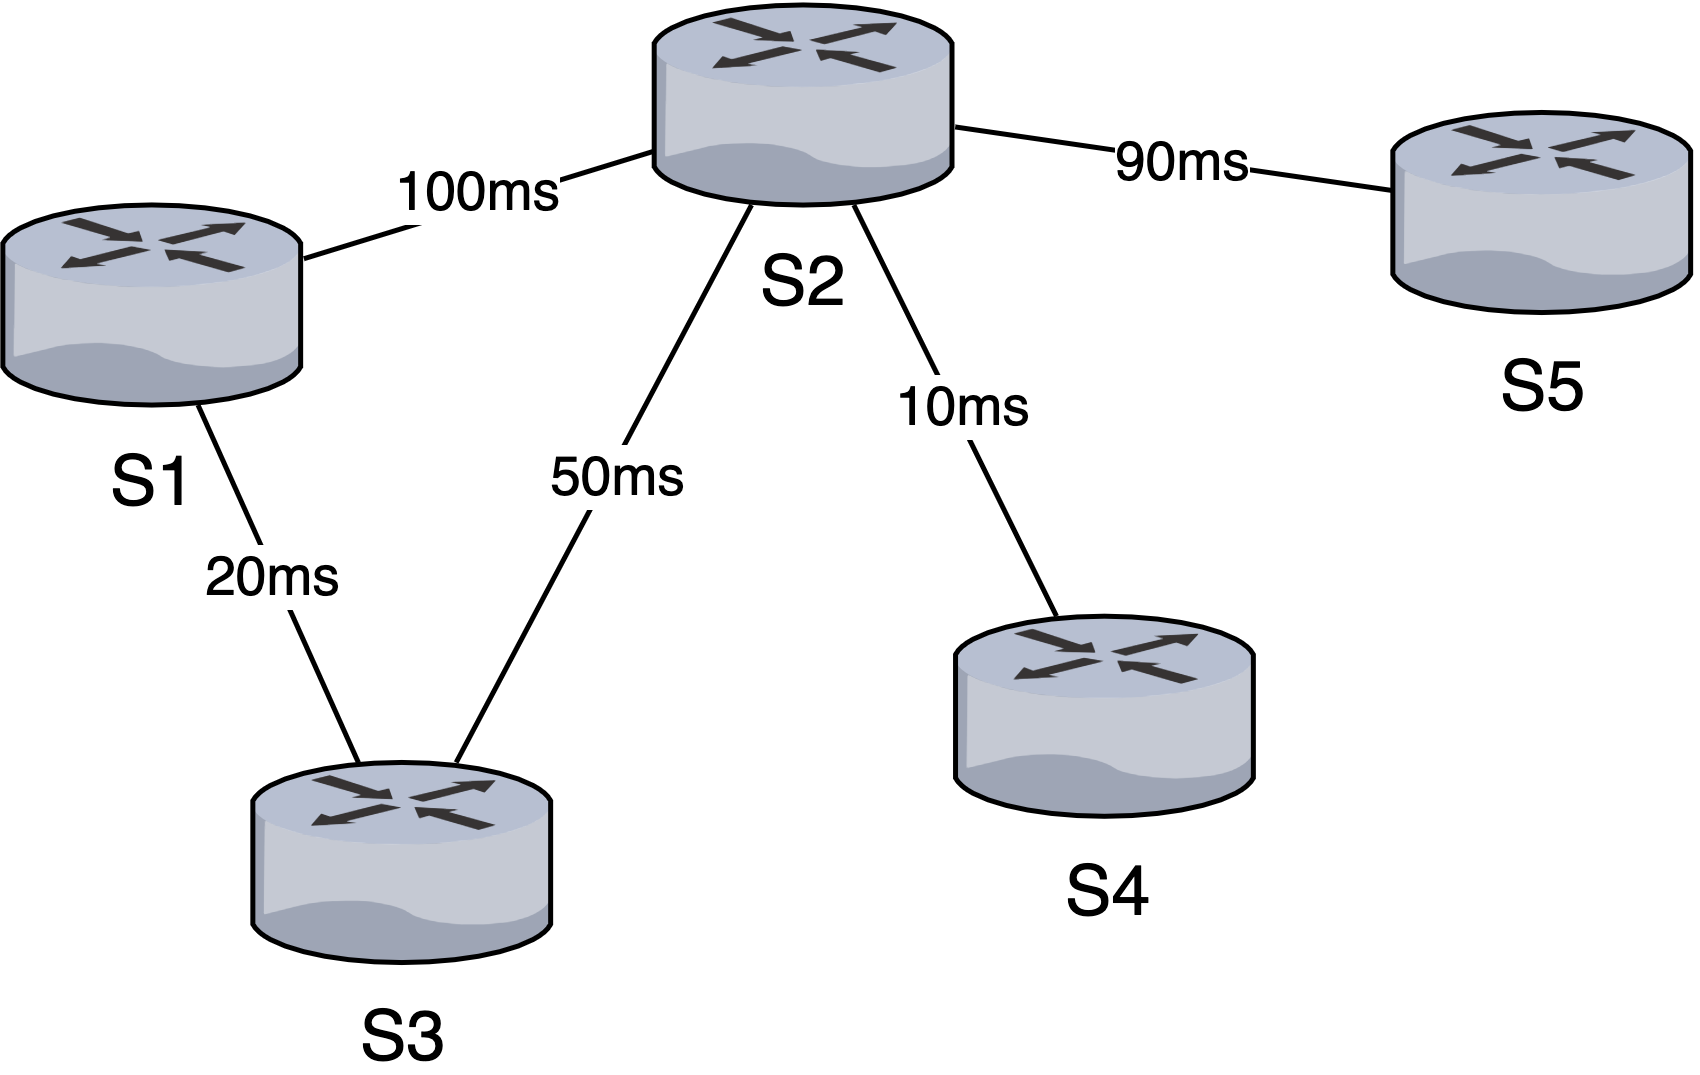
\includegraphics[width=0.5\textwidth]{./figures/ch4-simple-topo.png}}
\caption{简化后段路由节点相邻属性示意图}
\label{fig-ch4-simple-topo}
\end{figure}

\subsection{时延矩阵更新算法}

时延矩阵生成后,最重要的步骤是对时延矩阵进行更新,更新源数据的来源是本段路由节点对外部采集的时延结果和其他段路由节点组播通告结果。结果以键值对的方式存储,索引键为目的节点,值是探测节点到该目的节点的时延。

例如在图中,$S_1$主动探测可以获得$S_2$和$S_3$的时延信息,$S_2$可以获得$S_1, S_3, S_4, S_5$的时延信息,如下表所示:

\begin{table}[htbp]
\begin{tabular}{|p{0.2\textwidth}|p{0.7\textwidth}|}
\hline
1毫秒到10毫秒 & {[}{]} \\ \hline
10毫秒到100毫秒 & {[}S3:\{nil, 20ms\}{]} \\ \hline
100毫秒到1秒 & {[}S2:\{nil, 100ms\}{]} \\ \hline
\end{tabular}
\caption{S1主动探测获得的时延矩阵}
\label{table-S1-get}
\end{table}

$S_2$会将这几条时延信息通告给全网:

\begin{table}[htbp]
\begin{tabular}{|p{0.2\textwidth}|p{0.7\textwidth}|}\hline
1毫秒到10毫秒 & {[}{]} \\ \hline
10毫秒到100毫秒 & {[}S3:\{nil, 50ms\}, S4:\{nil, 10ms\}, S5:\{nil, 90ms\}{]} \\ \hline
100毫秒到1秒 & {[}S1:\{nil, 100ms\}{]} \\ \hline
\end{tabular}
\caption{S2通告的时延矩阵}
\label{table-S2-adverse}
\end{table}

$S_1$接收到这些信息后会将其更新在自己的时延矩阵中:

\begin{table}[htbp]
\begin{tabular}{|p{0.2\textwidth}|p{0.7\textwidth}|}\hline
1毫秒到10毫秒 & {[}{]} \\ \hline
10毫秒到100毫秒 & {[}S3:\{nil, 20ms\}{]} \\ \hline
100毫秒到1秒 & {[}S2:\{nil, 100ms\}, S4:\{S2, 110ms\}, S5:\{S2, 190ms\}{]} \\ \hline
\end{tabular}
\caption{S1接收S2公告后的时延矩阵}
\label{table-S1-after-S2}
\end{table}

在每组新的数据收到后,将执行时延矩阵更新算法,具体算法如下:

对每组数据进行可达性判断并加上沿途的时延,例如$S_1$收到$S_2$到$S_4$的时延是10毫秒时,检查自己没有$S_1$到$S_4$的时延记录,就讲$S_1$到$S_2$的时延和$S_2$到$S_4$的时延加在一起作为$S_1$到$S_4$的时延,并更新到100毫秒到1秒的时延矩阵中。需要注意的是如果本节点本身就对另一个节点可达,那么需要比较原本的方案和新生成的方案的时延,在时延矩阵中保留时延较短的方案。这样使得整个时延矩阵只会保留较小的时延方案,并不是所有的时延方案。

本节点将迭代相加直到更新本段路由节点到其他所有可达节点的时延,如果时延有降低则需要在算法的差分数据结构中进行遍历并对可以降级的时延和对应下一跳节点进行更新;如果时延有增高则需要在算法的差分数据结构中进行遍历并对需要升级的时延和对应的下一跳节点进行更新。当所有更新结束之后,就将新的时延矩阵组播或者广播通告出去。

\begin{figure}[htbp]
\setlength{\abovecaptionskip}{15pt plus 3pt minus 2pt}
\centerline{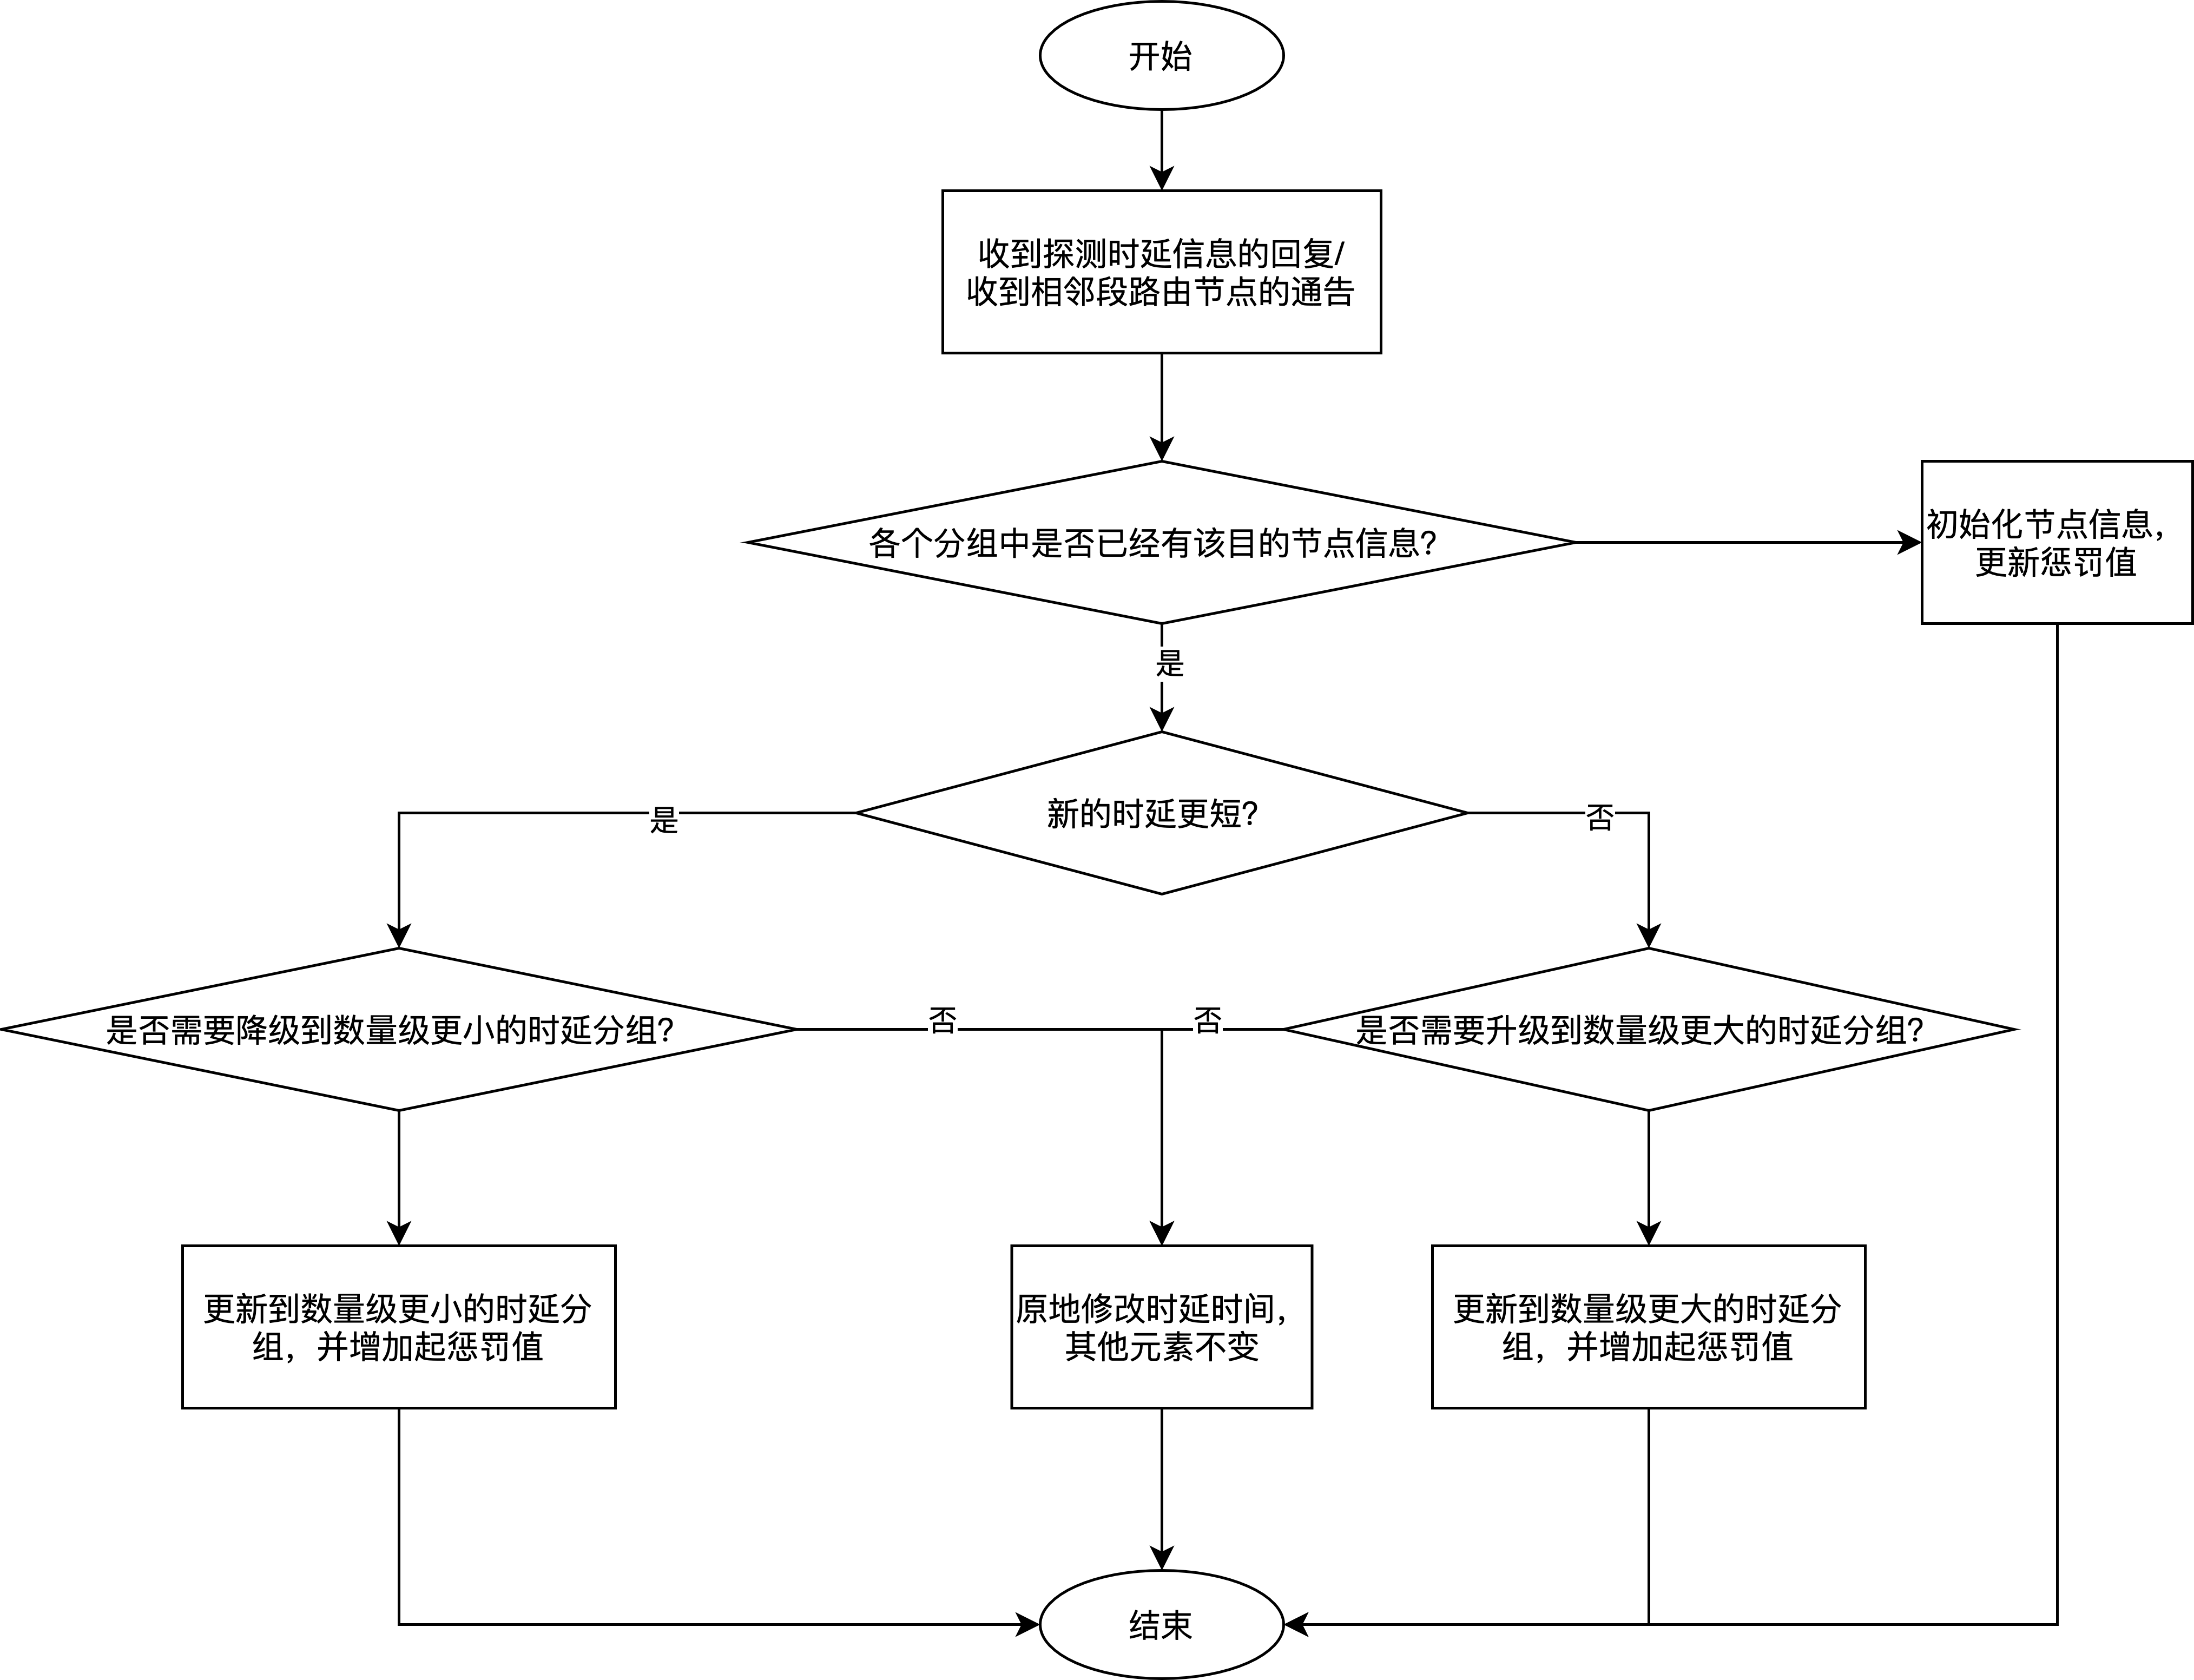
\includegraphics[width=1\textwidth]{./figures/ch4-sr-update.png}}
\caption{时延矩阵更新算法示意图}
\label{fig-ch4-sr-update}
\end{figure}

在使用段路由的较大规模网络中,由于段路由节点数目增多,段路由时延矩阵可能会变得变得十分庞大,这不光会使得存储时延矩阵将会占有大量的交换机内存资源,而且还会使得传输和处理段路由节点探测的时延信息所必需的带宽以及处理这些时延信息都需要大量的资源。因此考虑使用类似路由聚合(Routes Aggregation)的方式再时延矩阵更新算法中使用段路由节点聚合来减小段路由时延矩阵的规模,这是由于段路由节点其实是具有一定聚合的特性的,在第三章中使用的节点组中心度就是一个体现。另外通过对段路由节点的目的条目进行聚合,也可以隐藏一些过于详细的段路由节点时延信息,从而减少选路结果震荡对段路由网络带来的影响。

关于时延矩阵的更新有一个需要关注的挑战点,就是如何防止选路结果来回震荡。这是因为当一组段路由节点被选中的时候,这一组对应的时延就会增高,如果这个时候采集到了数据就很有可能对这个段路由节点的时延进行降级,而一旦这股流量结束了,采集到的时延就会降低,这个时候这个节点所属的差分时延组就会升级,而这样的变动可以看作是一种不稳定的体现,它这种在某组时延路由表中反复出现和消失就像是路由不稳定时表现出来的路由震荡,在网络中发生路由振荡时,路由器就会向邻居发布路由更新,收到路由更新报文的路由器需要重新计算路由并修改路由表。所以频繁的路由振荡会消耗大量的带宽资源和路由器CPU资源,严重时会影响到网络的正常工作。面对这样的情况,边界网关协议中有一个解决路由不稳定的思路,即路由衰减(Route Dampening)。多数情况下,边界网关协议都应用于复杂的网络环境中,路由变化十分频繁。为了防止持续的路由振荡带来的不利影响,边界网关协议使用路由衰减来抑制不稳定的路由。边界网关协议中使用惩罚值(Penalty Value)来衡量一条路由的稳定性,惩罚值的计算是当路由每发生一次振荡,边界网关协议便会给此路由增加一定的惩罚值(一般的做法是路由从激活状态变为未激活状态,惩罚值需要增加1000,路由在激活状态,收到新的路由更新,惩罚值加500),惩罚值越高就说明路由越不稳定。当惩罚值超过抑制阈值(Suppress Value)时,此路由被抑制,不加入到路由表中,也不再向其他边界网关协议对等体发布路由更新报文。而被抑制的路由每经过一段时间,惩罚值便会减少一半,这个时间称为半衰期(Half-life)。当惩罚值降到再使用阈值(Reuse Value)时,此路由变为可用并被加入到路由表中,同时向其他边界网关协议对等体发布路由更新报文。

参考边界网关协议的路由衰减机制,本章设计了对时延矩阵进行震荡抑制的方案,即有节点从不可达被加入时延矩阵时,惩罚值需要增加1000;每次有节点需要被升级或者降级的时候,就会给其惩罚值加500。并同样为其设置一个半衰期使得这个惩罚值可以随稳定时间增长而逐渐降低,本算法中的半衰期设置为往返时延与计算路由收敛时长和的两倍,实验中取1秒。与此同时当惩罚值到达800的抑制阈值时不可使用该段路由方案,直到降到200的重用阈值时可以开始使用,整个惩罚值随时间长度增长的变化趋势如图4-7所示,第2秒时新的段路由方案加入因此该方案当前惩罚值是1000,1秒的半衰期后降为500,第5秒和第7秒分别产生了该段路由方案在时延分组中的迁移,因此都增加了500的惩罚值,之后该段路由方案稳定,在第10秒的时候降低到重用阈值200以下开始可以被使用。

\begin{figure}[htbp]
\setlength{\abovecaptionskip}{15pt plus 3pt minus 2pt}
\centerline{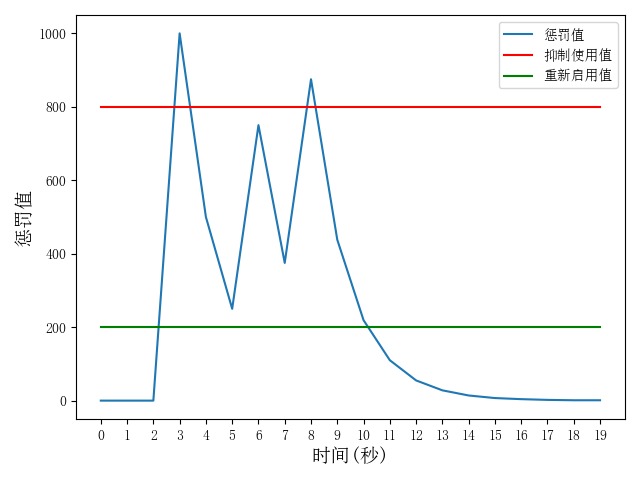
\includegraphics[width=0.6\textwidth]{./figures/ch4-penalty-value.png}}
\caption{惩罚值和半衰期随时间变化示意图}
\label{fig-ch4-penalty-value}
\end{figure}

而对于需要选择段路由航点列表方案的算法来说,在段路由节点列表的选择上则需要参考惩罚值,相同差分区域内进行段路由节点列表的选择时,会更倾向于选择惩罚值更低的段路由节点。

\subsection{段路由航点列表生成算法}

每个段路由节点将探测到的时延信息通告出去,并且所有节点的时延矩阵都趋近于收敛的时候,可以开始对服务流量开始执行选路算法。为简化问题,假设服务流量的源地址和目的地址都是段路由节点,这种假设实际上和真实网络中的情况有所出入,实际网络中源地址和目的地址一定都是主机的地址,但由于网络中的路由是按照网段进行最长前缀匹配路由的,所以可以按照交换机节点的位置选择流量调度的终点。因此段路由航点列表生成算法问题可以简化表达为对于一对段路由节点$S_i$和$S_j$,如何选择符合时延需求的段路由航点标签列表。

当带有时延请求的报文到达$S_i$时,$S_i$将在对应的差分段$[D_n^{start},D_n^{end}]$内寻找可行的方案,$D_n^{start}{<D}_{target}<D_n^{end}$,由于差分段内使用优先级队列进行存储,因此可以认为所有时延方案的排列是有序的,因此可以用二分法在$O\left(\sqrt n\right)$的时间内找到符合要求的方案。但是正好符合时延需求的方案大概率是不存在的,这里存在几种情况:第一种$[D_n^{start},D_n^{end}]$存在可行方案但是都比$D_{target}$大,这种情况下可以视网络具体情况而定,如果QPS较大,可以选择同一差分等级中当前时延最小的方案;如果QPS还比较小,也可以选择更短时延分段组内时延最大的方案,这意味着建立因此需要向上兼容选择时延较低的相邻方案,而且如果该业务的优先级很低也可以选择拒绝。第二种$[D_n^{start},D_n^{end}]$存在可行方案但是都比$D_{target}$小,那么直接选择这组内时延组大的方案即可。第三种是$\left[D_n^{start},D_n^{end}\right]$内不存在方案,那么处理方式和第一种一样。第四种就是最符合预期的方案$\left[D_n^{start},D_n^{end}\right]$内存在合适方案,且有比目标时延大的,也有比目标时延小的,此时按照二分法获取符合目标时延需求的方案即可。第五种则是每种分组时延的方案中都没有目的地址是$S_j$的方案,即$S_j$对于$S_i$来说不可达,可以直接拒绝服务请求。流程总结如图4-8所示。

\begin{figure}[htbp]
\setlength{\abovecaptionskip}{15pt plus 3pt minus 2pt}
\centerline{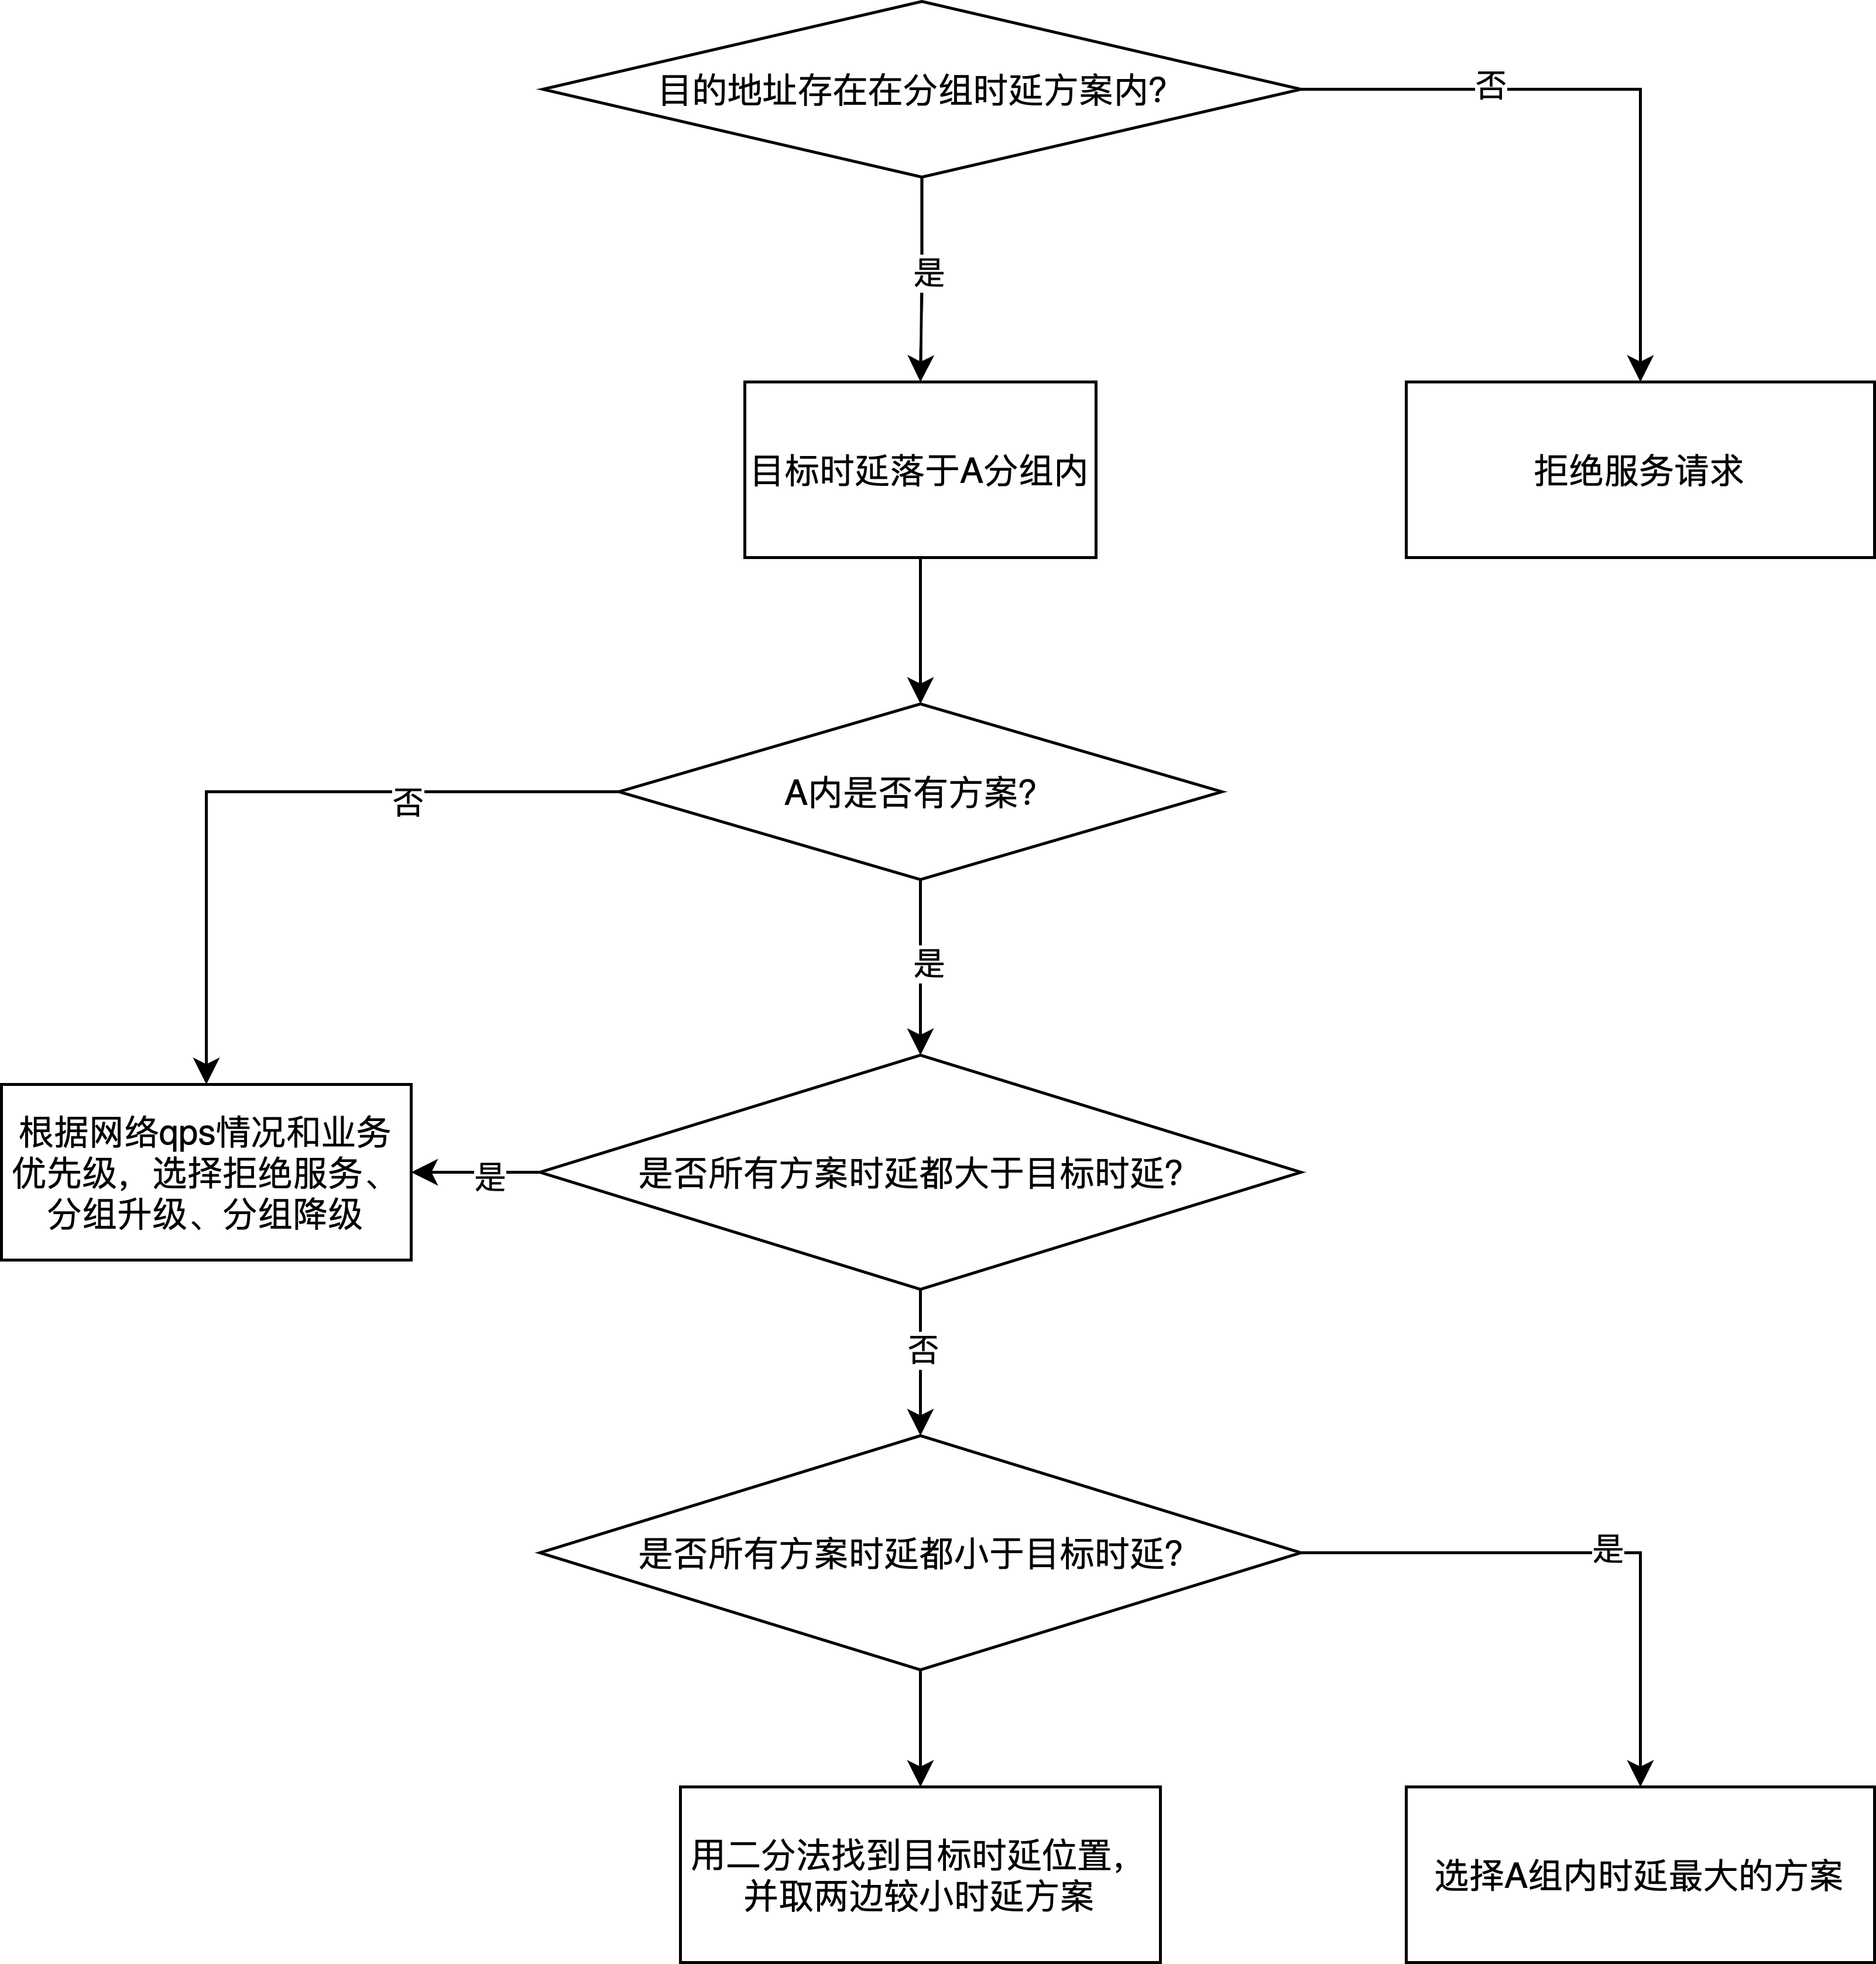
\includegraphics[width=0.9\textwidth]{./figures/ch4-find-sr-ans.png}}
\caption{段路由方案生成算法示意图}
\label{fig-ch4-find-sr-ans}
\end{figure}
    
确定选择的时延的方案后,就需要用递归的方式寻找整个段路由路径,例如$S_1$收到目的地知识$S_4$的报文,并且时延需求是150毫秒,那么在经过复杂化的下表中,首先定位到100毫秒到1秒的分组中,先通过哈希获取$S_4$方案的子列表头端点,最后通过二分法找到符合时延需求的段路由方案。在找到段路由方案之后,通过每组方案第一个元素代表的上一跳信息,逐步用递归的方式找到整个段路由列表。例如在下表中找到$S_4$之后,通过$S_4$的第一个元素$S_2$找到目的地址是$S_2$的方案,发现目的地址为$S_2$时下一跳时空,这说明已经递归完毕,可以返回整个段路由方案$S_1->S_2->S_4$。

\begin{table}[htbp]
\begin{tabular}{|p{0.2\textwidth}|p{0.7\textwidth}|}
\hline
1毫秒到10毫秒 & {[}{]} \\ \hline
10毫秒到100毫秒 & {[}S3:\{nil, 20ms\}{]} \\ \hline
100毫秒到1秒 & {[}S2:\{nil, 100ms\}, S4:\{S2, 110ms\}, S5:\{S2, 190ms\}{]} \\ \hline
\end{tabular}
\caption{S1时延矩阵}
\label{table-S1-delay-metric}
\end{table}

将上述算法总结为算法流程图如图4-9所示:

\begin{figure}[htbp]
\setlength{\abovecaptionskip}{15pt plus 3pt minus 2pt}
\centerline{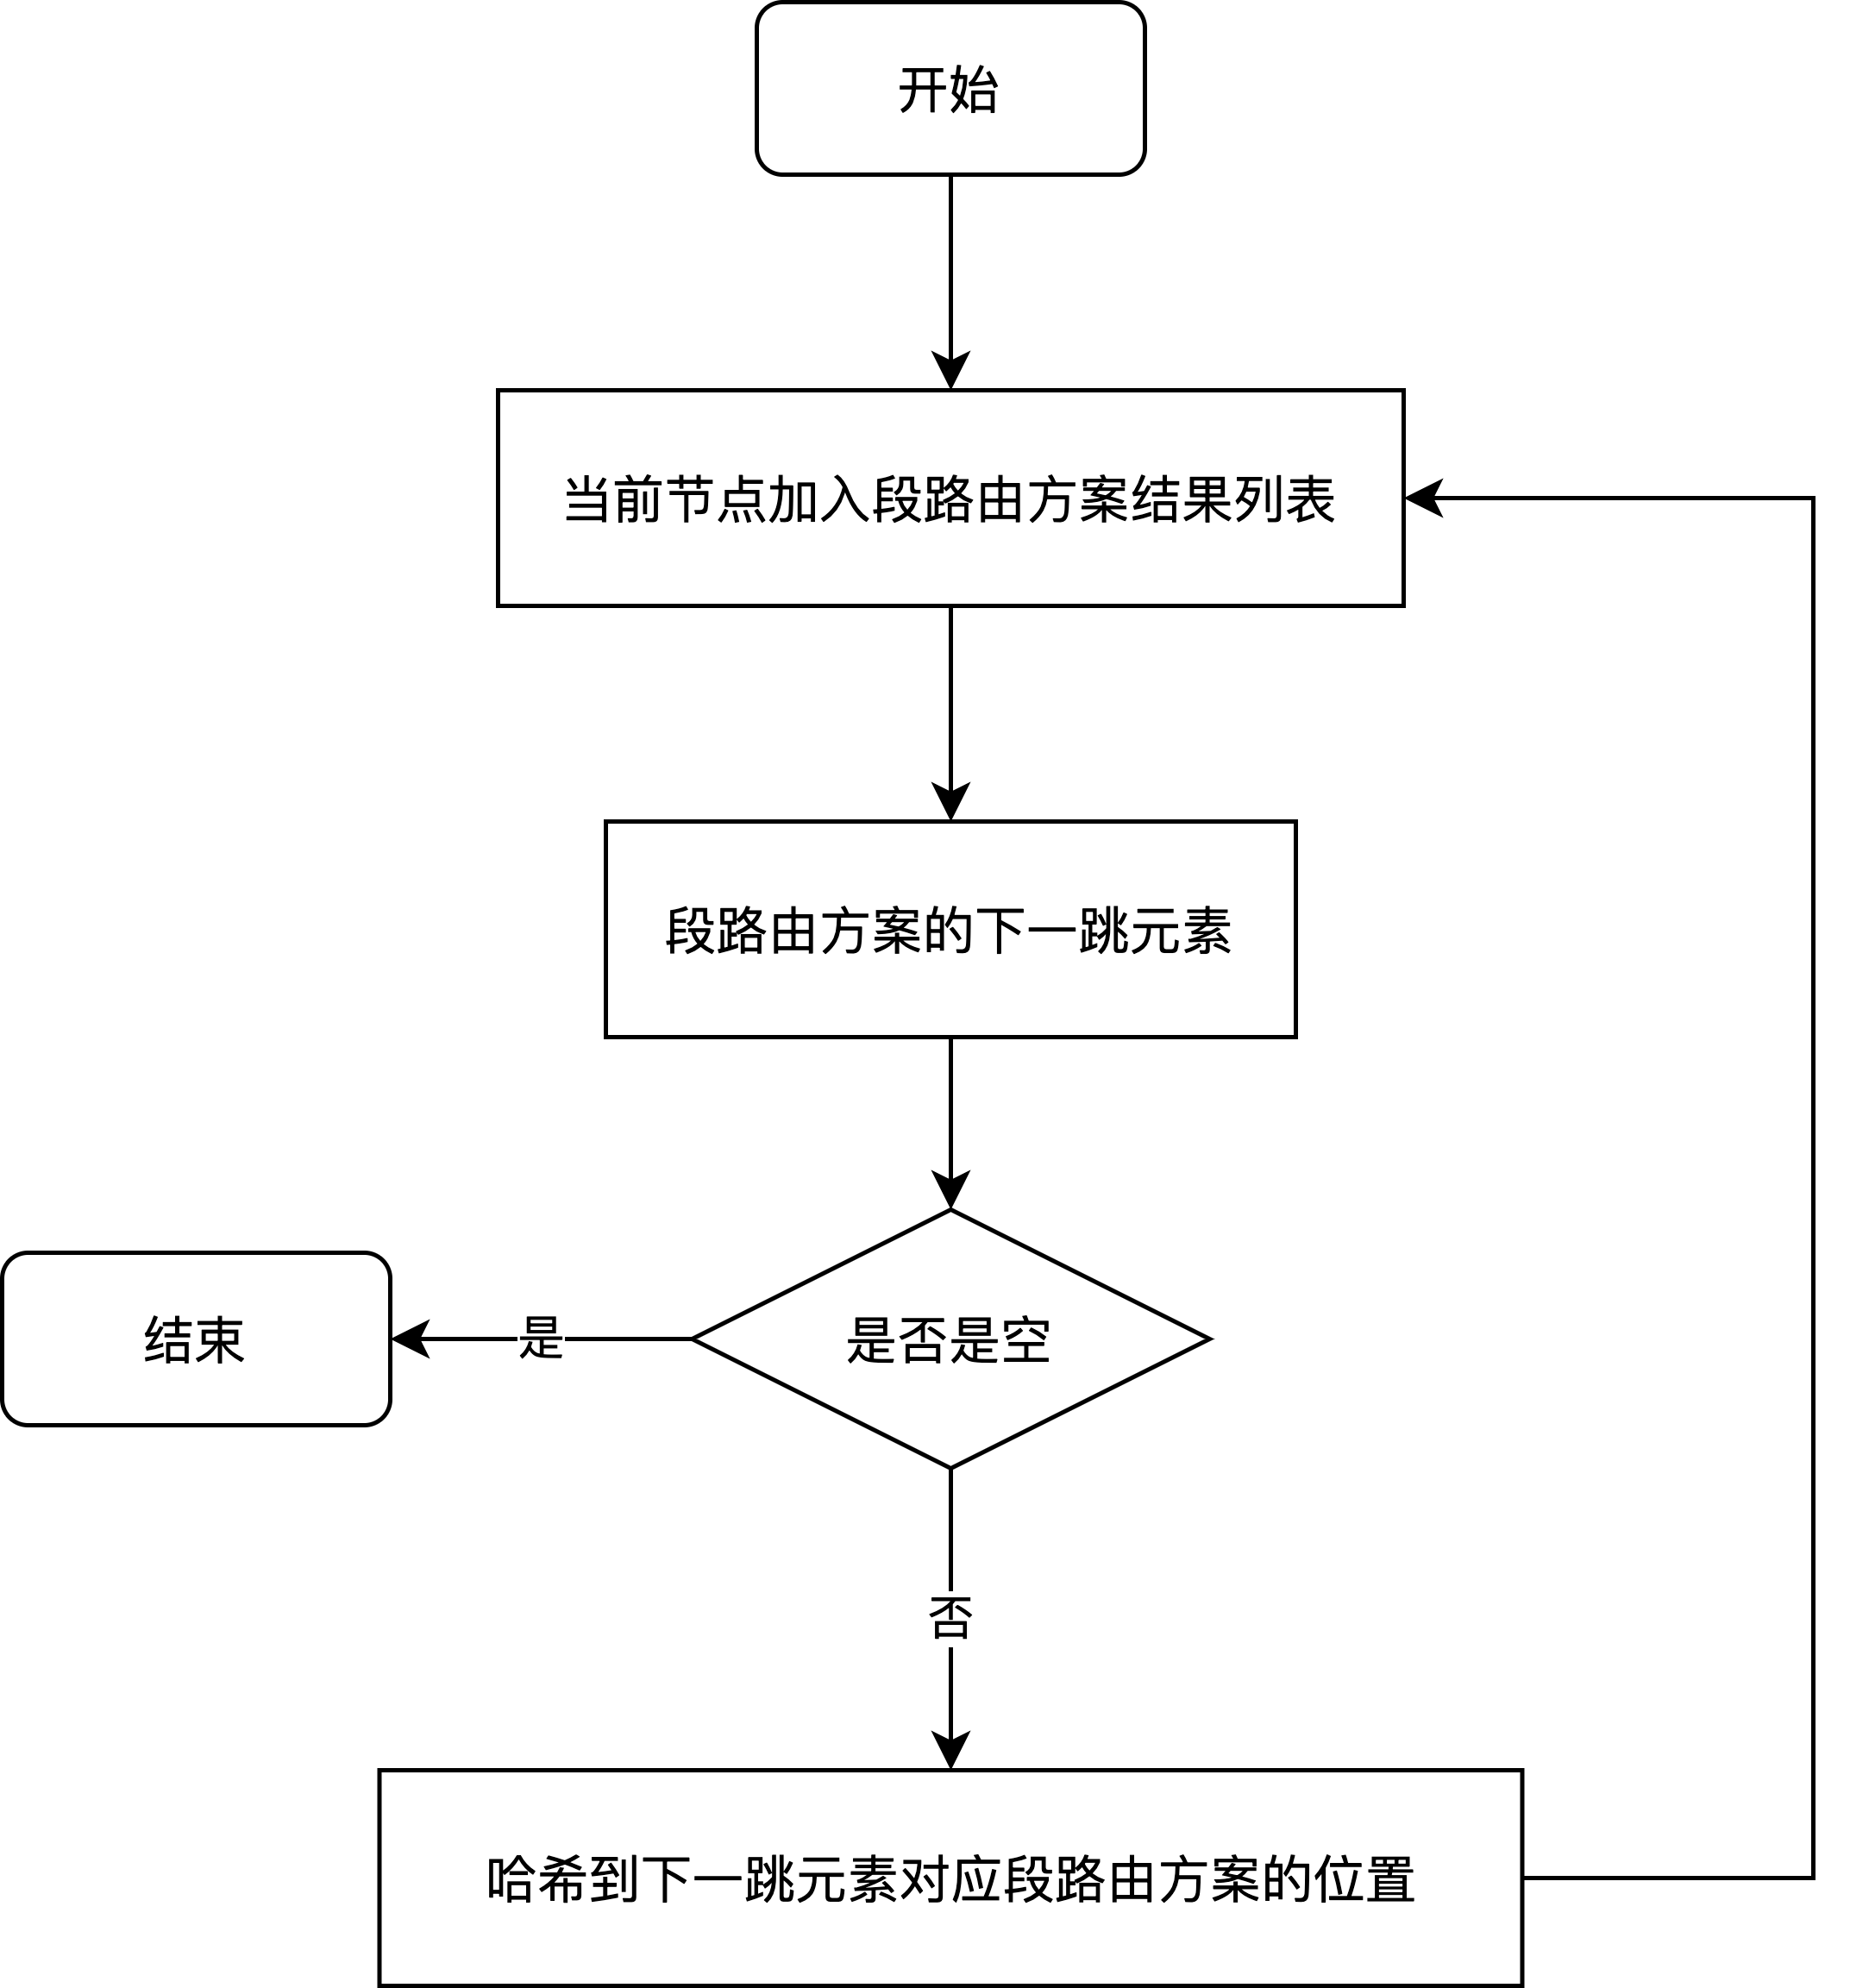
\includegraphics[width=0.6\textwidth]{./figures/ch4-sr-init.png}}
\caption{段路由标签列表生成算法示意图}
\label{fig-ch4-sr-init}
\end{figure}

\subsection{算法时间复杂度分析}

本章提出算法的时延复杂度如下:

时延矩阵更新算法需要遍历所有的方案,最好情况$O\left(1\right)$的时间复杂度,最差情况下具有$O\left(n\right)$的时间复杂度,因此平均时间复杂度为$O\left(n\right)$;段路由航点列表生成算法需要首先找到节点位置,最好情况下$O\left(1\right)$的时间复杂度,最差情况下$O\left(\sqrt n\right)$,平均时间复杂度为$O\left(\sqrt n\right)$;第二步生成整个段列表,只需要递归即可,最好情况下时间复杂度为$O\left(1\right)$,最差情况下需要递归到全部节点即$O\left(n\right)$,平均为$O\left(n\right)$。综上所述由于本章使用较多的哈希数据结构,使得整体时间复杂度较低。

\section{本章小结}

本章提出了一种分布式的段路由航点列表生成算法,用于在网络节点较多的广域网络中用分布式的方式提供基于段路由的低延迟路径流量调度服务。由于本章主要采用分布式,因此缺少了软件定义网络下控制器集中式的网络优化途径,但也正因为没有使用集中式控制器使得本章提出的算法可以较为简单地在更大的网络内直接部署。本章算法的核心在于差分时延矩阵的生成、更新和选择,本章对算法进行了详细的解释,并留出了一些参数可以在实验或者真实场景部署阶段进行调整,例如惩罚值的压制阈值等。最后该算法要求在使用时根据拓扑的情况配置段路由航点列表的长度限制,这是为了防止过长的段路由航点列表造成较低的链路有效负载和造成过多的端到端总跳数降低整个网络的吞吐量。

% 测试所有参考文献类型\cite{CITATION_BOOK,CITATION_ARTICLE,CITATION_PROCEEDINGS,CITATION_INPROCEEDINGS,CITATION_TECHREPORT,CITATION_STANDARD,CITATION_PATENT,CITATION_NEWSPAPER,CITATION_ELECTRONIC,SRSURVEYS}。

%% 本章参考文献
\ifx\usechapbib\empty
\nocite{BSTcontrol}
\setcounter{NAT@ctr}{0}
\bibliographystyle{buptgraduatethesis}
\bibliography{bare_thesis}
\fi
